
\documentclass[14pt]{extarticle}

\usepackage[T2A]{fontenc}
\usepackage[utf8]{inputenc}
\usepackage[english, russian]{babel}
\usepackage{url}
\usepackage{booktabs}
\usepackage{nicefrac}
\usepackage{microtype}
\usepackage{lipsum}
\usepackage{graphicx}
\usepackage{subfig}
\usepackage[square,sort,comma,numbers]{natbib}
\usepackage{doi}
\usepackage{multicol}
\usepackage{multirow}
\usepackage{tabularx}
\usepackage{tabulary}
\usepackage{pifont}
\usepackage{colortbl}

\usepackage{tikz}
\usetikzlibrary{matrix}
% Algorithms
\usepackage{algorithm}
\usepackage{algpseudocode}
\makeatletter
\renewcommand{\ALG@name}{Алгоритм}
\makeatother
%% Шрифты
\usepackage{euscript} % Шрифт Евклид
\usepackage{mathrsfs} % Красивый матшрифт
% \usepackage{extsizes}
\usepackage{makecell} % diaghead in a table
\usepackage{amsmath,amsfonts,amssymb,amsthm,mathtools,dsfont}
\usepackage{icomma}

\usepackage[center]{titlesec}
\usepackage{amsthm}
\usepackage{amssymb}
\usepackage{amsmath}
\usepackage{color}
\usepackage{wrapfig}
\usepackage{caption}
% \usepackage{subcaption}
\usepackage{indentfirst}
\usepackage[utf8]{inputenc} % allow utf-8 input
\usepackage[T1]{fontenc}    % use 8-bit T1 fonts
\usepackage{hyperref}       % hyperlinks
\usepackage{url}            % simple URL typesetting
\usepackage{booktabs}       % professional-quality tables
\usepackage{amsfonts}       % blackboard math symbols
\usepackage{nicefrac}       % compact symbols for 1/2, etc.
\usepackage{microtype}      % microtypography
\usepackage{xcolor}         % colors
\usepackage{stackrel}
\usetikzlibrary{matrix,arrows.meta,quotes,positioning}
\usetikzlibrary{calc}

\usepackage{hyperref}
\hypersetup{
	unicode=true,
	pdftitle={Generative causal inference approach to BCI analysis},
	pdfsubject={q-bio.NC, q-bio.QM},
	pdfauthor={Vladimirov Eduard Anatolevich},
	pdfkeywords={First keyword, Second keyword, More},
	colorlinks=true,
	linkcolor=black,        % внутренние ссылки
	citecolor=green,        % на библиографию
	filecolor=magenta,      % на файлы
	urlcolor=blue           % на URL
}

\usepackage{enumitem} % Для модификаций перечневых окружений
\usepackage{etoolbox}
\expandafter\patchcmd\csname\string\algorithmic\endcsname{\itemsep\z@}{\itemsep=1.5mm}{}{}

\usepackage{geometry}
\geometry{left=3cm}
\geometry{right=1.5cm}
\geometry{top=2.0cm}
\geometry{bottom=2.0cm}
\setlength\parindent{1.25cm}    % Устанавливает длину красной строки 15pt
\linespread{1.3}             % Коэффициент межстрочного интервала

\usetikzlibrary{arrows.meta}
\usetikzlibrary{quotes}

\def\ltrn{\mathcal{L}_{\mathrm{train}}}
\def\lval{\mathcal{L}_{\mathrm{val}}}

\newcommand\argmin{\mathop{\arg\min}}
\newcommand{\hchi}{\hat{\boldsymbol{\chi}}}
\newcommand{\hphi}{\hat{\boldsymbol{\varphi}}}
\newcommand{\bchi}{\boldsymbol{\chi}}
\newcommand{\A}{\mathcal{A}}
\newcommand{\B}{\mathcal{B}}
\newcommand{\x}{\mathbf{x}}
\newcommand{\hx}{\hat{x}}
\newcommand{\hy}{\hat{y}}
\newcommand{\M}{\mathcal{M}}
\newcommand{\N}{\mathcal{N}}
\newcommand{\R}{\mathbb{R}}
\newcommand{\p}{p(\cdot)}
\newcommand{\q}{q(\cdot)}
\newcommand{\uu}{\mathbf{u}}
\newcommand{\vv}{\mathbf{v}}
\newcommand{\bz}{\mathbf{z}}
\newcommand{\bx}{\mathbf{x}}
\newcommand{\by}{\mathbf{y}}
\newcommand{\bv}{\mathbf{v}}
\newcommand{\bw}{\mathbf{w}}
\newcommand{\ba}{\mathbf{a}}
\newcommand{\bb}{\mathbf{b}}
\newcommand{\bff}{\mathbf{f}}
\newcommand{\bh}{\mathbf{h}}
\newcommand{\bl}{\mathbf{l}}
\newcommand{\bp}{\mathbf{p}}
\newcommand{\bq}{\mathbf{q}}
\newcommand{\bs}{\mathbf{s}}
\newcommand{\bt}{\mathbf{t}}
\newcommand{\bu}{\mathbf{u}}
\newcommand{\bT}{\mathbf{T}}
\newcommand{\bX}{\mathbf{X}}
\newcommand{\bZ}{\mathbf{Z}}
\newcommand{\bS}{\mathbf{S}}
\newcommand{\bI}{\mathbf{I}}
\newcommand{\bH}{\mathbf{H}}
\newcommand{\bW}{\mathbf{W}}
\newcommand{\bY}{\mathbf{Y}}
\newcommand{\bU}{\mathbf{U}}
\newcommand{\bQ}{\mathbf{Q}}
\newcommand{\bP}{\mathbf{P}}
\newcommand{\bA}{\mathbf{A}}
\newcommand{\bB}{\mathbf{B}}
\newcommand{\bC}{\mathbf{C}}
\newcommand{\bE}{\mathbf{E}}
\newcommand{\bF}{\mathbf{F}}
\newcommand{\bK}{\mathbf{K}}
\newcommand{\bV}{\mathbf{V}}
\newcommand{\bsigma}{\boldsymbol{\sigma}}
\newcommand{\bSigma}{\boldsymbol{\Sigma}}
\newcommand{\bomega}{\boldsymbol{\omega}}
\newcommand{\btheta}{\boldsymbol{\theta}}
\newcommand{\bgamma}{\boldsymbol{\gamma}}
\newcommand{\bdelta}{\boldsymbol{\delta}}
\newcommand{\bPsi}{\boldsymbol{\Psi}}
\newcommand{\bpsi}{\boldsymbol{\psi}}
\newcommand{\bxi}{\boldsymbol{\xi}}
\newcommand{\bmu}{\boldsymbol{\mu}}
\newcommand{\bzeta}{\boldsymbol{\zeta}}
\newcommand{\blambda}{\boldsymbol{\lambda}}
\newcommand{\beps}{\boldsymbol{\varepsilon}}
\newcommand{\bZeta}{\boldsymbol{Z}}
% mathcal
\newcommand{\cX}{\mathcal{X}}
\newcommand{\cY}{\mathcal{Y}}
\newcommand{\cW}{\mathcal{W}}
\newcommand{\dH}{\mathds{H}}
\newcommand{\dR}{\mathds{R}}
% transpose
\newcommand{\T}{^{\mathsf{T}}}
% command to strike out text
\newcommand{\stkout}[1]{\ifmmode\text{\sout{\ensuremath{#1}}}\else\sout{#1}\fi}
\renewcommand{\epsilon}{\ensuremath{\varepsilon}}
\renewcommand{\phi}{\ensuremath{\varphi}}
\renewcommand{\kappa}{\ensuremath{\varkappa}}
\renewcommand{\le}{\ensuremath{\leqslant}}
\renewcommand{\leq}{\ensuremath{\leqslant}}
\renewcommand{\ge}{\ensuremath{\geqslant}}
\renewcommand{\geq}{\ensuremath{\geqslant}}
\renewcommand{\emptyset}{\varnothing}
\renewcommand{\baselinestretch}{1}

\newcommand{\vect}[1]{\boldsymbol{\mathbf{#1}}}
\newtheorem{theorem}{Theorem}[section]
\newtheorem{corollary}{Corollary}[theorem]
\newtheorem{lemma}[theorem]{Lemma}
\newtheorem{proposition}[theorem]{Proposition}
\newtheorem{assumption}[theorem]{Assumption}

\newtheorem{Th}{Теорема}
\newtheorem{Def}{Определение}
\newenvironment{Proof} % имя окружения
{\par\noindent{\bf Proof:}} % команды для \begin
{\hfill$\scriptstyle\blacksquare$} % команды для \end
\newtheorem{Assumption}{Предположение}
\newtheorem{Corollary}{Следствие}
\newtheorem{problem}{Problem}

\graphicspath{{../figures/}}

\renewcommand{\abstractname}{Аннотация}


\begin{document}
	\thispagestyle{empty}

\begin{titlepage}
	\begin{center}
		\textsc{Московский физико-технический институт}\\
		(национальный исследовательский университет)\\
		\textsc{Физтех-школа прикладной математики и информатики}\\
		\textsc{Кафедра интеллектуальных систем}
	\end{center}
	\vspace{2.5cm}
	\begin{center}
		{Владимиров Эдуард Анатольевич}
		\par
		\vspace{2cm}
		{\Large \textsc{\textbf{Причинно-ориентированное снижение размерности для анализа данных нейроинтерфейсов}}}
		\par
		\vspace{2cm}
		{09.04.01 ~--- Информатика и вычислительная техника}
		\par
		\vspace{2cm}
		\textsc{Выпускная квалификационная работа магистра}
	\end{center}
	\vspace{2cm}
	\hfill\parbox{8,4cm}{\textbf{Научный руководитель:}
		\\д.ф.-м.н. В.\,В.\,Стрижов}
	\par
	\vspace{2cm}
	\begin{center}
		{Москва~--- 2025}
	\end{center}
\end{titlepage}
	
	\newpage
	\tableofcontents
	\newpage
	
%	\begin{abstract}
%		Learning low–dimensional representations that preserve cause–and–effect structure is a key step toward interpretable modelling of high-dimensional dynamical data.
%		This thesis introduces \textbf{CaSCA}, a linear auto-encoder that splits the latent space into a causal block, capturing delayed directed influence from one multivariate series to another, and a reconstructive block, keeping residual variance.  
%		Extensions to trajectory embeddings, Riemannian covariance spaces, and a deep variant with a differentiable Convergent Cross Mapping loss broaden the framework.  
%		Comprehensive experiments on two real-world datasets—dual accelerometer-gyroscope recordings and EEG–IMU traces of table-tennis sessions—show that CaSCA  
%		(i) reduces multicollinearity,  
%		(ii) reconstructs signals with negligible loss of explained variance, and  
%		(iii) improves downstream prediction
%		The method thus offers a compact, interpretable state-space where causal links are easier to detect and exploit.
%		
%		\bigskip
%		\textbf{Keywords}: \emph{dimensionality reduction, causal representation learning, canonical correlation analysis, state space reconstruction, EEG, IMU, Riemannian geometry, convergent cross mapping}
%	\end{abstract}

\begin{abstract}
	Изучение низкоразмерных представлений, сохраняющих причинно–следственную структуру, является ключевым шагом на пути к интерпретируемому моделированию многомерных динамических данных.
	В тезисе представлен линейный автокодировщик \textbf{CaSCA}, который разбивает скрытое пространство на каузальный блок, фиксирующий отложенное направленное влияние от одного многомерного ряда к другому, и реконструктивный блок, сохраняющий остаточную дисперсию.  
	Расширения для траекторных эмбеддингов, римановых ковариационных пространств и нейросетевого варианта с дифференцируемым методом сходящегося перекрёстного отображения расширяют фреймворк.  
	Вычислительный эксперимент на двух реальных наборах данных ~-- записях с использованием двух акселерометров и гироскопа и ЭЭГ—ИИМ, полученных во время игры в настольный теннис, ~-- показывают, что CaSCA  
	(i) уменьшает мультиколлинеарность,
	(ii) восстанавливает сигналы с незначительной потерей объясняемой дисперсии и  
	(iii) улучшает последующее прогнозирование.
	Таким образом, метод предлагает компактное, поддающееся интерпретации пространство состояний, в котором причинно-следственные связи легче обнаруживать и использовать.
	
	\bigskip
	\textbf{Ключевые слова}: \emph{уменьшение размерности, изучение причинно-следственных связей, канонический корреляционный анализ, реконструкция пространства состояний, ЭЭГ, риманова геометрия, конвергентное перекрестное отображение}.
\end{abstract}
	
	\newpage
	
	\section{Introduction}
	
	Identifying directed causal links among components of a dynamical system is central to many scientific domains, such as neuroscience, climate science, and economics.
	True understanding requires more than correlation: one needs a representation that makes causal mechanisms explicit and testable.  
	Classic tools such as linear Granger causality \citep{Granger1969} and transfer entropy \citep{Schreiber2000} check whether past values of one series improve the prediction of another.  
	Yet they operate in the raw measurement space, assume fixed linear effects, and struggle when high dimensionality, nonlinear coupling, or evolving dynamics hide the signal in noise.  
	These limitations lead to ``mirage correlations’’ that appear and vanish with changing regimes \citep{Sugihara2012}, while the curse of dimensionality dilutes statistical power in large sensor arrays \citep{Runge2019}
	
	A growing body of work therefore shifts attention from \emph{discovery in the original space} to \emph{learning a low-dimensional state space} in which causal relations become tractable.  
	State–space reconstruction unfolds the attractor of a dynamical system so that nearby points share similar futures, providing a geometrically faithful arena for causal tests.  
	Recent advances in causal representation learning \citep{Scholkopf2021} confirm that suitable embeddings can disentangle latent drivers and thus sharpen downstream inference.  
	
	Building on these ideas we propose \textbf{CaSCA} ~--- Causal Subspace Canonical Analysis ~--- a family of causal dimensionality-reduction methods that balance the variance-preserving objective of PCA with the cross-predictive focus of CCA.  
	The key hypothesis is that causal influence is concentrated in a subspace of the hidden state and that separating this \emph{causal} subspace from a purely \emph{reconstructive} subspace yields more interpretable and predictive models.  
	CaSCA retains essential dynamical variance and explicitly tests whether the extracted causal coordinates improve auto-regressive prediction of target variables.  
	Three complementary quality criteria guide the evaluation: variance-inflation metrics for collinearity, reconstruction error for information retention, and forecast skill for causal utility.  
	
	We demonstrate CaSCA on two time-series settings of increasing complexity.  
	First, ten-minute accelerometer–gyroscope recordings from two wearable devices illustrate how shared latent dynamics can be captured by a few causal components that transfer across sensors.  
	Second, EEG–IMU recordings of table-tennis players show that Riemannian trajectory embeddings coupled with CaSCA improve the classification of successful versus failed hits.  
	Across both cases we compare causality assessed in the original space with causality assessed in the learned state space and find consistent gains in interpretability and predictive power.  
	
	To extend CaSCA beyond linear projections we outline two modifications.  
	Working in \emph{trajectory space} embeds lagged blocks instead of instantaneous samples, capturing delayed effects without exponential parameter growth.  
	A \emph{Riemannian variant} projects covariance trajectories onto the manifold of symmetric positive-definite matrices, respecting the intrinsic geometry of neural data.  
	Finally, we sketch a deep learning extension in which a cross-attention encoder replaces linear CCA and a differentiable Convergent Cross Mapping loss imposes monotonic cross-map convergence during training.  
	
	The contributions of this thesis are fourfold.  
	First, we formalise causal dimensionality reduction as the joint optimisation of reconstruction and cross-predictive objectives.  
	Second, we introduce CaSCA and prove that, under generic observability and weak-noise conditions, its causal subspace recovers the true latent drivers up to rotation.  
	Third, we provide empirical evidence that causal analysis in the learned state space outperforms traditional pipelines in both explanatory clarity and forecasting accuracy.  
	Fourth, we deliver open-source implementations that support linear, Riemannian, and neural variants of the framework.  
	
	The remainder of the thesis is organised as follows.  
	Section~\ref{sec:causal-dim-red} reviews causal representation learning and dimensionality-reduction methods.  
	Section~\ref{sec:ssr} surveys state-space reconstruction techniques that motivate our choice of embedding.  
	Section~\ref{sec:problem} formulates the problem and introduces the evaluation criteria.  
	Section~\ref{sec:purecca} details the CaSCA algorithm.  
	Section~\ref{sec:mods} presents the trajectory-space, Riemannian, and deep extensions.  
	Section~\ref{sec:experiments} reports computational experiments on the wearable and EEG–IMU datasets.  
	Section~\ref{sec:future} outlines future directions, and Section~\ref{sec:conclusion} concludes.  
	
	\section{Literature review}
	
	\subsection{Causal Representation Learning} \label{sec:causal-dim-red}
	High–dimensional observations rarely reveal causal structure directly.  
	Causal representation learning therefore seeks a mapping
	\[
	R:\;\dR^{p} \longrightarrow \dR^{d},
	\qquad d\ll p,
	\]
	such that the image coordinates preserve the mechanisms that generate the data.  
	The central difficulty is identifiability: many maps can reconstruct the observations, but only a few (sometimes only one) respect the underlying cause–effect relations.  
	This section reviews the main methodological lines that have attacked that challenge.
	
	\subsubsection*{Linear mixture models}
	
	The earliest identifiable setting assumes each observable is an instantaneous linear mixture of statistically independent, non-Gaussian “sources’’  
	\[
	\mathbf{x} = A \,\mathbf{s}, \qquad A \in \dR^{p\times p}.
	\]
	Higher–order statistics pin down $A^{-1}$ up to scaling and permutation; ICA algorithms \citep{lee1998independent} exploit this fact to produce latent candidates for causal factors.  
	LiNGAM \citep{Shimizu2006} embeds ICA inside a linear, acyclic Structural Equation Model (SEM), rewriting the mixture as  
	\[
	\mathbf{x}=B^{\top}\mathbf{x}+\boldsymbol\varepsilon,
	\]
	where the upper–triangular weight matrix $B$ encodes directed edges and $\boldsymbol\varepsilon$ is i.i.d.\ non-Gaussian noise.  
	Because the permutation freedom in ICA coincides with the causal ordering, the full DAG becomes identifiable.  
	\textsc{DirectLiNGAM} \citep{Shimizu2011} replaces the iterative ICA step with a deterministic finite-search procedure, making the approach computationally robust.
	
	\paragraph{Scope and limits.}
	When all assumptions — linearity, non-Gaussianity, no latent confounding — are correct, LiNGAM provides an exact, interpretable causal representation.  
	Once Gaussian noise, feedback loops, or unmeasured common causes enter, identifiability collapses; extensions such as Latent‐LiNGAM repair only special cases.  
	
	\subsubsection*{Supervised linear projections}
	
	Pure PCA \citep{abdi2010principal} maximises variance and risks projecting away low-variance but causally crucial directions.  
	Sufficient–dimension‐reduction (SDR) methods instead require that a projection $B^{\top}\mathbf{x}$ retain the conditional distribution of an outcome $Y$:
	\[
	Y\;\perp\!\!\!\perp\;\mathbf{x}\;\bigl|\;B^{\top}\mathbf{x}.
	\]
	In the causal vocabulary, $B$ must preserve all paths from $\mathbf{x}$ to $Y$.  
	Canonical Correlation Analysis (CCA) and its time-lagged version TL-CCA realise this principle when variables arrive in two "views" — e.g. putative causes and effects separated by a lag \citep{Moneta2023}.  
	Granger-PCA rotates ordinary principal axes so that each component predicts future values as strongly as possible, thereby ranking latent directions by dynamical influence as well as variance.
	
	\paragraph{Scope and limits.}
	Linear SDR is fast, transparent, and easy to bias with domain knowledge (e.g.\ fix directions known to be causal).  
	Because correlation does not imply causation, these projections must be interpreted with care: they preserve causal signal only if the analyst steers them toward it.
	
	\subsubsection*{Temporal models}
	
	Time furnishes a partial ordering: causes precede effects.  
	Vector-autoregressive LiNGAM extends the linear non-Gaussian framework to lagged interactions, recovering both instantaneous and delayed edges in a single estimation scheme.  
	When linearity is doubtful or dimensionality large, constraint–based algorithms such as PCMCI/PCMCI $+$ \citep{Runge2019}, \citep{runge2020discovering} test conditional independences across lags, pruning indirect and common-driver links while controlling false positives under autocorrelation.  
	These procedures effectively yield a low-dimensional set of lagged parents for each variable—a dynamic causal representation.
	
	\paragraph{Scope and limits.}
	Temporal precedence can break many equivalences that plague static data, yet non-stationarity, seasonality or strong feedback still confuse tests and require long records.  
	Moreover, hidden variables active at multiple lags can masquerade as direct links, reminding the analyst that time order alone does not guarantee completeness.
	
	\subsubsection*{Nonlinear neural models}
	
	To handle image, audio or raw sensor data one embeds causal assumptions inside deep generative models.  
	CausalVAE inserts a learnable DAG layer between independent exogenous latents $z_0$ and dependent latents $z$, then decodes $z$ to reconstruct $\mathbf{x}$ \citep{Yang2021}.  
	An acyclicity penalty keeps the latent graph well-behaved, and interventions on any latent dimension propagate through the decoder to produce counterfactual observations.  
	Recent theory shows that, given multiple environments that perturb the latent noise terms, such models can recover causal latents up to permutation and scaling \citep{Scholkopf2021}.
	
	\paragraph{Scope and limits.}
	Deep causal models accommodate arbitrary nonlinearity and high-dimensionality, but they trade closed-form guarantees for optimisation stability and the availability of multi-environment data.  
	Without strong inductive bias, the learnt representation may still conflate causal and spurious factors.
	
	\subsubsection*{Summary}
	
	Over the past thirty years, methods have evolved from simple linear models that work under strict assumptions to complex deep‐learning approaches that need a lot of data and conditions to hold.  
	Linear mixture methods use non‐Gaussian signals to find causes, supervised projections like PCA/CCA keep information relevant to a target, time‐series algorithms use the order of events, and neural networks can learn rich causal features if given data from different settings.  
	Our method, \textbf{CaSCA}, sits in the middle: it uses straightforward PCA/CCA ideas but forces the chosen components to capture causal relationships and make good predictions with time lags.  
	In this way, it aims to produce a low‐dimensional representation that is easy to understand and still preserves the true causal links, without relying on overly restrictive assumptions.  
	
	\subsection{State Space Reconstruction}\label{sec:ssr}
	
	\textbf{State-space reconstruction (SSR)} refers to the process of constructing a multi-dimensional phase space from time-series data such that the dynamics of an unknown system can be studied in that space. 
	Even if a few variables of a dynamical system are observed, SSR aims to recover the underlying state trajectory  in a reconstructed state-space that is diffeomorphic to the true state-space of the system.
	evolving on an attractor $\mathcal{A}$ whose fractal dimension is $d_A$.  
	
	Let $(M, \varphi^t)$ be a smooth, compact manifold of dimension $d_A$, with flow
	
	$$
	\varphi^t\colon M\;\to\;M\,,\qquad x(t)=\varphi^t(x_0)\,,
	$$
	
	and let the observation function be
	
	$$
	h\colon M\;\to\;\dR^s, 
	$$
	
	so the time series data is a function $$ y(t)\;=\;h\bigl(x(t)\bigr). $$
	
	\subsubsection*{Time–Delay Embedding}
	
	Following Packard \citep{Packard1980} and Takens \citep{Takens1981}, construct the delay‐coordinate map:
	
	$$
	\Psi_{E,\tau}\colon M\;\to\;\dR^E,
	\quad
	\Psi_{E,\tau}\bigl(x(t)\bigr)
	=\Bigl(y(t),\,y(t-\tau),\,y(t-2\tau),\dots,y\bigl(t-(E-1)\tau\bigr)\Bigr).
	$$
	
	Takens’ theorem states that, for a generic $h$ and any smooth flow on an attractor of dimension $d_A$, if $E > 2\,d_A,$ then $\Psi_{E,\tau}$ is an embedding (i.e.\ ae diffeomorphism onto its image).
	
	Under the embedding $\Psi_{E,\tau}$, attractor dimension and lyapunov exponents are preserved.
	
	\subsubsection*{Singular Spectrum Analysis (SSA)}
	
	\textbf{Singular Spectrum Analysis} is a method that combines delay embedding with linear decomposition techniques to extract modes of variability from a time series \citep{Broomhead1986,Vautard1992,Golyandina2001}. It can be seen as a data-driven, nonparametric spectral decomposition method, closely related to \textit{principal component analysis} (PCA) on time-delay vectors. In SSA, one first forms the Hankel matrix of the time series using a chosen window length $L$. For a series $X = (x_1, \dots, x_N)$, the trajectory matrix is: 
	
	$$ 
	\mathbf{X} = [\,X_1 : X_2 : \cdots : X_K\,] \;\in \dR^{L \times K}, \quad \text{where } X_i = (x_i, x_{i+1}, \dots, x_{i+L-1})^T, 
	$$ 
	
	and $K = N - L + 1$. 
	Next, SSA performs a \textit{singular value decomposition} (SVD) of this trajectory matrix: $\mathbf{X} = \sum_{j=1}^L \sqrt{\lambda_j}\,U_j V_j^T$.
	Equivalently, it diagonalizes the $L\times L$ lag-covariance matrix $\mathbf{S} = \mathbf{X}\mathbf{X}^T$ to obtain eigenvalues $\lambda_1 \ge \lambda_2 \ge \cdots \ge \lambda_L$ and eigenvectors $U_j$.
	The eigenvectors $U_j$ provide an orthonormal basis of the $L$-dimensional embedding space, and projecting the trajectory matrix onto each $U_j$ yields the principal components (also called temporal EOFs in SSA literature). 
	
	The final steps involve \textbf{grouping} and \textbf{reconstruction}: one groups subsets of these components (e.g. those corresponding to a signal or trend of interest) and computes a reduced-rank approximation of $\mathbf{X}$. From this approximated trajectory matrix, the time series is reconstructed by averaging along the diagonals (each anti-diagonal corresponds to one time index).
	By appropriate grouping, one can separate the original series into a sum of interpretable components: e.g. a slowly varying trend, oscillatory modes (often appearing as pairs of nearly equal $\lambda_j$ for sinusoidal components), and residual noise
	
	\subsubsection*{Manifold–Learning Embeddings}
	
	Classical delay embeddings and SSA use linear or fixed transformations. \textbf{Manifold learning} techniques, developed largely in the 2000s, enable nonlinear dimensionality reduction. \citep{roweis2000nonlinear}
	These methods attempt to discover a low-dimensional manifold on which the high-dimensional data lie, preserving intrinsic geometric structure.
	The key idea is that if the system has an attractor of dimension $d$, the data (in some embedding space) essentially lie on an $d$-dimensional manifold $\mathcal{M}$, and algorithms can learn coordinates on $\mathcal{M}$ that flatten out the nonlinear twists of the attractor.
	
	Common manifold learning algorithms include Locally Linear Embedding (LLE), Isomap, t-SNE, UMAP \citep{roweis2000nonlinear, balasubramanian2002isomap, van2008visualizing, mcinnes2018umap}.
	These are unsupervised algorithms that take a set of data points in a high-$D$ space and produce coordinates in a lower $d$-dimensional space.
	They typically construct a graph or neighborhood relations among the data points and then optimize some objective to preserve local distances or global geodesic structure.
	
	When applying these to time-series, a typical approach is: first, embed the time series in latent space to get a point cloud $\{y(t)\}$ that samples the attractor.
	Then run a manifold learning algorithm on $\{y(t)\}$.
	The result will be a set of coordinates $\{\xi(t)\}$ in $\dR^d$ that parametrizes the data manifold.
	Ideally, $d$ will equal the true attractor dimension or a useful reduced dimension.
	
	\subsubsection*{Riemannian and Geometric Representations}
	Another modern avenue for SSR involves representing segments of time series as geometric objects like covariance matrices or subspaces, which lie on curved manifolds. 
	The motivation is that certain features of dynamical systems -- especially in high-dimensional or multivariate settings -- are naturally encoded by covariance or subspace structure, and by considering the appropriate geometry one can better compare and analyze these features.
	
	\paragraph{SPD–covariance manifold.}  
	Given a $d$-dimensional multivariate time series or a $d$-channel signal and an embedding dimension $D$, one can form $D$-lagged vectors as before: $s_e(t) = [s_1(t), ..., s_d(t),\; s_1(t+\tau),...,s_d(t+\tau),\;\dots,\;s_1(t+(D-1)\tau),...,s_d(t+(D-1)\tau)]^T \in \dR^{dD}$.
	This is essentially a phase-space reconstruction applied to each channel \citep{pennec2006intrinsic}.
	From a window of such vectors, one can compute a \textbf{sample covariance matrix} $R = \frac{1}{N}\sum_{i=1}^N s_e(t_i) s_e(t_i)^T$, which will be a $dD \times dD$ SPD matrix (symmetric positive-definite).
	This covariance encapsulates both the spatial correlations between channels and temporal correlations up to lag $(D-1)\tau$.
	Each SPD matrix can be seen as a representation of the local state dynamics.
	By comparing SPD matrices from different time windows, one can quantify similarity of dynamical states.
	In practice, this approach has been very successful in scenarios like EEG where the true state is high-dimensional and noisy; the covariance provides a robust signature of the state that filters out high-frequency noise.
	This idea—popularised in BCI by \citet{barachant2013classification}.
	
	\paragraph{Grassmannian subspaces.}  
	Instead of the full covariance, one can represent the subspace spanned by certain vectors associated with the time series.
	A prime example: in SSA or subspace system identification, we obtain an orthonormal basis of principal components (or an observability subspace) for the dynamics.
	The column space spanned by, say, the first $r$ singular vectors $U_1,\dots,U_r$ of the trajectory matrix is an $r$-dimensional subspace of $\dR^L$.
	This subspace itself can be treated as a point on a Grassmann manifold $\mathcal{G}(r, L)$, which is a set of all $r$-dimensional subspaces in $\dR^L$.
	The Grassmann manifold has a natural Riemannian metric (derived from principal angles between subspaces), so one can measure distances between two subspaces.
	This concept is used in subspace-based clustering of time series and in linear system identification: each linear dynamical system of order $r$ corresponds to an $r$-dimensional observability subspace \citep{hamm2008grassmann,turaga2011statistical}.
	By embedding an unknown system’s data and estimating an $r$-dim subspace, one effectively reconstructs a linear state-space.
	Clustering on Grassmann then groups systems with similar subspaces.
	Recent reviews categorize various Grassmannian methods for multivariate time series clustering and modeling, highlighting that many algorithms differ by how they construct the subspace (e.g., via SVD of Hankel matrix, via autoregressive model subspace, or via frequency domain) but ultimately compare subspaces on $\mathcal{G}$.
	
	\subsubsection*{Summary}
	
	Traditional methods like time‐delay embedding and singular spectrum analysis let us rebuild the system’s attractor from a single observed variable so that the hidden dynamics become explicit.  
	Modern techniques add flexibility: nonlinear manifold learning finds lower‐dimensional coordinates that keep the attractor’s shape, while Riemannian methods use covariance or subspace geometry to compare complex states.  
	CaSCA relies on these reconstructed state spaces to extract a small set of components that capture causal influence, since working in the state domain makes cause‐and‐effect links easier to separate than in the raw measurement space.  
	Each SSR approach has its own assumptions, benefits, and drawbacks (see Table \ref{tab:ssr_selected}). In practice, we choose the one that best reveals the latent dynamics before applying CaSCA.
	
	\begin{table}[bhtp]
		\centering
		\renewcommand{\arraystretch}{1.25} % uniform row height
		\begin{tabularx}{\textwidth}{
				>{\raggedright\arraybackslash}p{3.3cm}   % fixed‑width first column
				>{\raggedright\arraybackslash}X           % assumptions
				>{\raggedright\arraybackslash}X           % strengths
				>{\raggedright\arraybackslash}X}          % limitations
			\toprule
			\textbf{Method} & \textbf{Assumptions} & \textbf{Strengths} & \textbf{Limitations} \\
			\midrule
			\textbf{Time-delay embedding} &
			deterministic, low-dimensional system; long and clear time series;  &
			simple; model-free; provably diffeomorphic reconstruction &
			parameter sensitivity and noise amplification \\[0.3em] \hline
			
			\textbf{Singular Spectrum Analysis} &
			$-$ &
			data-driven decomposition &
			linear reconstruction; parameter choices \\[0.3em] \hline
			
			\textbf{Manifold learning-based embeddings} &
			data lie on a smooth, low‑dimensional manifold; there is a large set of sample points &
			nonlinear dimensionality reduction &
			computational complexity ($O(N^2)$ or worse); no dynamics explicit; sensitive to kernel scale and neighbourhood choice; diffeomorphic equivalence is not guaranteed \\[0.3em] \hline
			
			\textbf{Riemannian \& geometric approaches} &
			relevant information about the state resides in second-order statistics or in a linear subspace of some feature space; dynamics captured via geodesic distances or curvature tensors &
			robustness; reduced complexity &
			information loss; not one-to-one; geometric complexity \\
			\bottomrule
		\end{tabularx}
		\caption{Concise comparison of selected state‑space reconstruction methods.}
		\label{tab:ssr_selected}
	\end{table}
	
	\section{Problem statement} \label{sec:problem}
	
	Let
	\[
	\mathbf X_t = \bigl[X_t^1, \ldots, X_t^{n_x}\bigr]\T, \qquad \mathbf Y(t)=\bigl[Y_t^1, \dots, Y_t^{n_y}\bigr]\T,
	\quad t=1, \dots, T,
	\]
	be two multivariate time series recorded at uniform sampling rate.
	We assume the observations are generated by an unknown nonlinear dynamical system that evolves on a compact attractor of finite dimension. The dependency between X and Y could be nonlinear and time-delayed.
	
	Next, we introduce a pair of shared encoders  
	\[
	\varphi_{\text{enc}}:\dR^{n_x}\times \dR^{n_y} \longrightarrow \dR^{m},
	\qquad
	\psi_{\text{enc}}: \dR^{n_x}\times  \dR^{n_y} \longrightarrow \dR^{m},
	\]
	applied row-wise to obtain latent matrices  
	\[
	\bP_t=\varphi_{\text{enc}}\bigl(\bX_t, \bY_t\bigr) \in \dR^{m},
	\qquad
	\bQ_t=\psi_{\text{enc}} \bigl(\bX_t, \bY_t\bigr) \in \dR^{m},
	\qquad
	t=1,\dots ,T.
	\]
	Two decoders  
	\[
	\varphi_{\text{dec}}: \dR^{m} \longrightarrow \dR^{n_x},
	\qquad
	\psi_{\text{dec}}: \dR^{m} \longrightarrow \dR^{n_y}
	\]
	map the embeddings back to reconstructions 
	
	Reconstructions are received by applying decoders to the latent projections:
	\[
	\widehat \bX_t = \varphi_{\text{dec}}(\varphi_{\text{enc}}(\bX_t, \bY_t)),
	\qquad
	\widehat \bY_t = \psi_{\text{dec}}(\psi_{\text{enc}}(\bX_t, \bY_t))
	\]
	
	The $m$ latent dimensions are partitioned into
	\[
	m=d_{\mathrm c}+d_{\mathrm r}, \qquad d_{\mathrm c}\ll m\ll min(n_x, n_y),
	\]
	where the first $d_{\mathrm c}$ coordinates form the \textbf{causal subspace} and the remaining $d_{\mathrm r}$ coordinates form the \textbf{reconstructive subspace}.  
	Formally,
	\[
	\bP_t=
	\begin{bmatrix}
		\bP_t^{\mathrm c} \\ \bP_t^{\mathrm r}
	\end{bmatrix},
	\quad
	\bQ_t=
	\begin{bmatrix}
		\bQ_t^{\mathrm c} \\ \bQ_t^{\mathrm r}
	\end{bmatrix},
	\qquad
	\bP_t^{\mathrm c}, \bQ_t^{\mathrm c} \in \dR^{d_{\mathrm c}},
	\quad
	\bP_t^{\mathrm r}, \bQ_t^{\mathrm r} \in \dR^{d_{\mathrm r}} .
	\]
	
	The first block is intended to capture the
	lagged causal interaction between $\bX_t$ and $\bY_t$, whereas the remaining
	coordinates are responsible for reconstruction.
	
	\paragraph{Meta-objective.}
	Learning jointly tunes encoder and decoders by minimising
	\[
	\mathcal L
	=
	\underbrace{\lambda_{\mathrm{rec}}
		\bigl[
		|| \bX_t - \widehat \bX_t ||_F + || \bY_t - \widehat \bY_t ||_F
		\bigr]}_{\text{reconstruction loss}}
	\;+\;
	\underbrace{\lambda_{\mathrm{c}}
		\,\mathcal L_{\mathrm c}\bigl(P_{t-\tau}^{\mathrm c},Q_t^{\mathrm c}\bigr)}_{\text{causal loss}},
	\]
	where  
	
	\begin{itemize}[leftmargin=1.4cm]
		\item $\mathcal L_{\mathrm c}$ is a \emph{causal alignment loss} that rewards statistical dependence between lagged causal embeddings  
		(for example, negative CCA correlation or negative CCM score);
		\item $\tau$ is a set of candidate time lags  
		$\tau \in \{0,1,\dots,\tau_{\max}\}$ that lets us detect after how many steps $\bX_{t - \tau}$ influences $\bY_t$;
		\item $\lambda_{\mathrm{rec}}, \; \lambda_{\mathrm{c}}>0$ balance reconstruction quality and causal fit.
	\end{itemize}
	
	As a result of this optimization, we obtain
	$\mathbf P_t^{\mathrm c}, \mathbf Q_t^{\mathrm c}$ — low-dimensional causal embeddings, and 
	$\widehat{\bX_t}, \widehat{\bY_t}$ — accurate reconstructions of the original signals.
	
	\paragraph{Constraints.}
	\begin{itemize}[nosep,leftmargin=1.2cm]
		\item The attractor is assumed to admit a delayed embedding under moderate noise.
		\item All significant causal information is contained in the subspace of dimension $d_{\mathrm c}$.
		\item The blocks $\bP^{\mathrm c}_t$ and $\bP^{\mathrm r}_t$ 
		(and likewise for $bQ_t$) are approximately orthogonal, reducing interference between reconstruction and causal analysis.
	\end{itemize}
	
	\subsection{Quality criteria.} \label{subsec:quality}
	\paragraph{Multicolinearity diagnostics.}
	For latent representations  $\bP_t, \; \bQ_t$
	we evaluate 
	\[
	\text{VIF} = \max_{j} \text{VIF}_j = \max_{j}\frac{1}{1-R_j^{2}},
	\quad
	\kappa = \frac{\sigma_{\max}}{\sigma_{\min}},
	\]
	where $R_j^{2}$ is the coefficient of determination when
	regressing the $j$-th column to the rest,
	and $\sigma_{\max},\sigma_{\min}$ are singular values
	of $\bP_t\T \bP_t$ and $\bQ_t\T \bQ_t$.
	
	\paragraph{Reconstruction error.}
	Only the first part of the losses is taken into account
	\(
	\mathcal L_{\mathrm{rec}}
	=
	\Vert\bX-\widehat\bX\Vert_F
	+
	\Vert\bY-\widehat\bY\Vert_F .
	\)
	
	\paragraph{Predictive performance.}
	For every downstream task we train three competing predictors:
	
	\begin{enumerate}[label=(\roman*),nosep,leftmargin=1.4cm]
		\item \( \mathcal{M}_{\mathrm{self}} \) that uses only the past of the target,  
		\( \bF^{(i)}_t = \bigl\{ \bY_{t}\bigr\}_{\tau\in\mathcal{T}} \);
		\item \( \mathcal{M}_{\mathrm{raw}} \) that augments those lags with the raw driver series,  
		\( \bF^{(ii)}_t = \bigl\{ \bY_{t},\,\bX_{t-\tau}\bigr\}_{\tau\in\mathcal{T}} \);
		\item \( \mathcal{M}_{\mathrm{causal}} \) that replaces the raw driver by the causal embedding,  
		\( \bF^{(iii)}_t = \bigl\{ \bY_{t},\,\bP_{t-\tau}^{\mathrm c}\bigr\}_{\tau\in\mathcal{T}} \).
	\end{enumerate}
	
	Let \(\mathrm{Perf}(\mathcal{M})\) denote the chosen evaluation metric  
	(negative RMSE for regression, or F1-score for classification).  
	The relative gain provided by the causal features is quantified by
	\[
	\Delta_{\text{score}}
	\;=\;
	\mathrm{Perf}\bigl(\mathcal{M}_{\mathrm{causal}}\bigr)
	\;-\;
	\max\Bigl\{
	\mathrm{Perf}\bigl(\mathcal{M}_{\mathrm{self}}\bigr),\,
	\mathrm{Perf}\bigl(\mathcal{M}_{\mathrm{raw}}\bigr)
	\Bigr\}.
	\]
	
	A positive \(\Delta_{\text{score}}\) indicates that the causal subspace
	\(\bP^{\mathrm c}\) yields better predictions than any combination
	of the original observables, thus validating the utility of causal embeddings.
	
	
	\section{Suggested Method CaSCA} \label{sec:purecca}
	
	CaSCA is a linear two–block encoder–decoder that separates a pair of
	multivariate time–series \(\{\bX_t ,\bY_t\}_{t=1}^{T}\) into
	\emph{causal coordinates}, responsible for the directed lagged influence
	\(\bX_{t-\tau}\!\to\bY_t\), and \emph{reconstructive coordinates}, which
	retain the remaining variance.  
	All steps are algebraic (CCA\,+\,PCA); no gradient optimisation is
	required.
	
	%------------------------------------------------------------
	\subsection*{Lag autodetection by shifted CCA}
	
	Choose a candidate set of lags
	\(\mathcal{T}=\{0,1,\dots,\tau_{\max}\}\).  
	For each \(\tau\in\mathcal{T}\) centre the data,
	form the shifted pairs
	\(\bX_{t-\tau},\,\bY_t\) (dropping incomplete rows), run one–component
	CCA, and record the canonical correlation \(\rho(\tau)\).  
	The maximiser
	\[
	\tau^{\star}=\arg\max_{\tau\in\mathcal{T}}\rho(\tau)
	\]
	is used in all subsequent formulas.
	
	%------------------------------------------------------------
	\subsection*{Causal part}
	
	\begin{enumerate}[leftmargin=1.4cm,label=(C\arabic*)]
		\item
		Fit CCA with \(d_{\mathrm c}\) components to the
		pair \((\bX_{t-\tau^{\star}},\bY_t)\).  
		Let the CCA weight matrices be
		\[
		\bW_x^{\mathrm c}\in\dR^{n_x\times d_{\mathrm c}},
		\qquad
		\bW_y^{\mathrm c}\in\dR^{n_y\times d_{\mathrm c}}.
		\]
		\item
		Construct the causal scores at all time steps
		\[
		\bP_t^{\mathrm c}= \bX_{t-\tau^{\star}}\,\bW_x^{\mathrm c},
		\qquad
		\bQ_t^{\mathrm c}= \bY_t\,\bW_y^{\mathrm c}.
		\]
		\item Remove the rank-\(d_{\mathrm c}\) causal projection
		\[
		\bX_{\text{res}}
		= \bX_t - \bP_t^{\mathrm c}{\bW_x^{\mathrm c}}\T,\quad
		\bY_{\text{res}}
		= \bY_t - \bQ_t^{\mathrm c}{\bW_y^{\mathrm c}}\T,
		\]
	\end{enumerate}
	
	\subsection*{Reconstruction part}
	
	\begin{enumerate}[leftmargin=1.4cm,label=(R\arabic*)]
		\item
		Apply PCA with \(d_{\mathrm r}=m-d_{\mathrm c}\) components to each
		residual and collect
		\[
		\bW_x^{\mathrm r}\in\dR^{n_x\times d_{\mathrm r}},
		\qquad
		\bW_y^{\mathrm r}\in\dR^{n_y\times d_{\mathrm r}}.
		\]
		\item
		Define the reconstructive scores
		\[
		\bP_t^{\mathrm r}= \bX_{res}\,\bW_x^{\mathrm r},
		\qquad
		\bQ_t^{\mathrm r}= \bY_{res}\,\bW_y^{\mathrm r}.
		\]
	\end{enumerate}
	
	%------------------------------------------------------------
	
	Every centred observation is expressed as the sum of its two
	orthogonal parts
	\[
	\widehat{\bX}_t
	=\overline{\bX}
	\;+\;
	\bP_t^{\mathrm c}{\bW_x^{\mathrm c}}^{\!\mathsf T}
	\;+\;
	\bP_t^{\mathrm r}{\bW_x^{\mathrm r}}^{\!\mathsf T},
	\qquad
	\widehat{\bY}_t
	=\overline{\bY}
	\;+\;
	\bQ_t^{\mathrm c}{\bW_y^{\mathrm c}}^{\!\mathsf T}
	\;+\;
	\bQ_t^{\mathrm r}{\bW_y^{\mathrm r}}^{\!\mathsf T},
	\]
	where \(\underline{\bX},\underline{\bY}\) are the column means.
	
	%------------------------------------------------------------
	\subsection*{Theoretical properties in the whitened space}
	Let the centred and whitened data matrices be
	\[
	X\!\in\!\R^{T\times n_x},\;
	\Sigma_{xx}=\frac{1}{T}X^{\top}X = I_{n_x}
	\].
	CaSCA returns two orthonormal loading sets  
	\(W_x^{\mathrm c}\in\R^{n_x\times d_{\mathrm c}}\)  
	and \(W_x^{\mathrm r}\in\R^{n_x\times d_{\mathrm r}}\)
	with \(d_{\mathrm c}+d_{\mathrm r}=d_{\mathrm hid}\).
	Their score blocks are
	
	\[
	P^{\mathrm c}=X\,W_x^{\mathrm c}\in\R^{T\times d_{\mathrm c}},
	\quad
	P^{\mathrm r}=X\,W_x^{\mathrm r}\in\R^{T\times d_{\mathrm r}}.
	\]
	
	Note, that by the construction $W_x^{\mathrm c}, W_x^{\mathrm r}, W_y^{\mathrm c}, W_y^{\mathrm r}$ are column-wise orthogonal: by construction for PCA weights and by whittening for CCA weights.
	
	%--------------------  LEMMA  ---------------------
	\begin{lemma}[Score orthogonality]\label{lem:score_orth}
		After whitening, the causal and reconstructive scores are Euclidean-orthogonal:
		\[
		P^{\mathrm c\!\top}\,P^{\mathrm r}=0_{d_{\mathrm c}\times d_{\mathrm r}}.
		\]
	\end{lemma}
	
	\begin{Proof}
		The causal projector is \(P_c=W_x^{\mathrm c}{W_x^{\mathrm c}}^{\!\top}\).
		By construction of the residual we have  
		\(X_{\mathrm{res}} = X - X\,P_c\) and
		\(P^{\mathrm r}=X_{\mathrm{res}}W_x^{\mathrm r}\).
		Using the whitened inner product,
		
		\[
		\!P^{\mathrm c\!\top}P^{\mathrm r}
		= W_x^{\mathrm c\!\top}X^{\top}\bigl(X-XP_c\bigr)W_x^{\mathrm r}
		= W_x^{\mathrm c\!\top}(I_{n_x}-P_c)W_x^{\mathrm r}
		= W_x^{\mathrm c\!\top}W_x^{\mathrm r}-W_x^{\mathrm c\!\top}P_cW_x^{\mathrm r}
		= 0.
		\]
	\end{Proof}
	
	Define the score–covariance blocks
	\[
	\Sigma_{pp}^{\mathrm{cc}}
	:=\frac1T P^{\mathrm c\!\top}P^{\mathrm c}\in\R^{d_{\mathrm c}\times d_{\mathrm c}},\;
	\Sigma_{pp}^{\mathrm{rr}}
	:=\frac1T P^{\mathrm r\!\top}P^{\mathrm r}\in\R^{d_{\mathrm r}\times d_{\mathrm r}}.
	\]
	
	%------------------  THEOREM  ---------------------
	\begin{theorem}[CaSCA Euclidean block structure]
		\label{thm:orth_blocks}
		In the whitened space the following hold.
		\begin{enumerate}[label=(\roman*)]
			\item \emph{Weight orthogonality:}
			\({W_x^{\mathrm c}}^{\!\top}W_x^{\mathrm r}=0_{d_{\mathrm c}\times d_{\mathrm r}}\).
			\item \emph{Score orthogonality:}
			\(P^{\mathrm c\!\top}P^{\mathrm r}=0\)  (Lemma~\ref{lem:score_orth}).
			\item \emph{Additive covariance decomposition:}
			\[
			\Sigma_{xx}=W_x^{\mathrm c}\,\Sigma_{pp}^{\mathrm{cc}}\,{W_x^{\mathrm c}}^{\!\top}
			+W_x^{\mathrm r}\,\Sigma_{pp}^{\mathrm{rr}}\,{W_x^{\mathrm r}}^{\!\top}.
			\]
		\end{enumerate}
	\end{theorem}
	
	\begin{Proof}
		\textbf{(i)}  PCA on \(X_{\mathrm{res}}\) is performed after an
		explicit Gram–Schmidt step against \(W_x^{\mathrm c}\), therefore the
		column spaces are orthogonal.
		
		\textbf{(ii)}  Stated and proved in Lemma~\ref{lem:score_orth}.
		
		\textbf{(iii)}  Using the additive expansion
		\(X = P^{\mathrm c}{W_x^{\mathrm c}}^{\!\top} + P^{\mathrm r}{W_x^{\mathrm r}}^{\!\top}\),
		
		\[
		\Sigma_{xx}
		=\tfrac1T X^{\top}X
		= W_x^{\mathrm c}\Sigma_{pp}^{\mathrm{cc}}{W_x^{\mathrm c}}^{\!\top}
		+W_x^{\mathrm r}\Sigma_{pp}^{\mathrm{rr}}{W_x^{\mathrm r}}^{\!\top}
		+\underbrace{W_x^{\mathrm c}
			\tfrac1T P^{\mathrm c\!\top}P^{\mathrm r}}_{=0}
		{W_x^{\mathrm r}}^{\!\top}
		+\underbrace{W_x^{\mathrm r}
			\tfrac1T P^{\mathrm r\!\top}P^{\mathrm c}}_{=0}
		{W_x^{\mathrm c}}^{\!\top},
		\]
		where the cross terms vanish by (ii).
	\end{Proof}
	
	The theorem confirms that, after whitening (or equivalently using a
	$\Sigma$-aware projector), CaSCA splits the total variance into two
	independent, orthogonal blocks.
	The reconstruction follows directly:
	\[
	\widehat X_t
	= \;\overline{X}\;+\;
	P_t^{\mathrm c}{W_x^{\mathrm c}}^{\!\top}
	+P_t^{\mathrm r}{W_x^{\mathrm r}}^{\!\top},
	\]
	and analogously for \(\widehat Y_t\).
	
	\paragraph{Consequences.}
	Whitening or the equivalent Mahalanobis projector yields  
	\emph{strict Euclidean orthogonality} between causal and reconstructive
	loadings, an \emph{additive variance decomposition}, and guarantees that
	down-stream regressors can use the two latent blocks without
	multicollinearity.  
	If whitening is skipped these properties still hold in the Mahalanobis
	metric defined by \(\Sigma_{xx}\) and \(\Sigma_{yy}\).
	
	\bigskip
	\noindent
	CaSCA therefore delivers a compact latent representation with (i) an
	automatically chosen causal delay, (ii) an interpretable split between
	directed and residual variance, and (iii) provable orthogonality after a
	single, inexpensive whitening step.
	
	\section{Modifications} \label{sec:mods}
	\subsection{CaSCA in a Takens–trajectory space}\label{subsec:purecca-traj}
	
	The linear formulation of \textsc{CaSCA} operates on the raw sensor
	vectors $\bx_t\in\R^{n_x}$ and $\by_t\in\R^{n_y}$.  
	When the underlying dynamics are nonlinear, however, those vectors
	represent only low–dimensional projections of a larger deterministic
	state and may hide the causal geometry that drives the
	interaction.\footnote{See Section~\ref{sec:ssr} for a full review of
		state-space reconstruction.}  
	A common remedy is to \emph{lift every time-stamp into a
		short trajectory}: a time–delay embedding that unfolds the local
	manifold and renders cross–dependencies more linear and
	time-aligned.
	
	\paragraph{Delay coordinates.}
	Fix embedding orders $p,q\!\in\!\N$ and spacing $\tau>0$.  
	For each timestamp $t$ construct the
	\emph{trajectory vectors}
	\[
	\widehat{\bX}_t \;=\;
	\bigl[\bX_t,\,\bX_{t-1},\dots,\bX_{t-q+1}\bigr]\T\in\R^{q n_x},
	\quad
	\widehat{\bY}_t \;=\;
	\bigl[\bY_t,\,\bY_{t-1},\dots,\bY_{t-p+1}\bigr]\T\in\R^{p n_y}.
	\]
	Under the classical Takens conditions with $q>\!2d_\A$ (and
	analogously for $p$) the map
	$t\!\mapsto\!(\widehat{\bX}_t,\widehat{\bY}_t)$ is a diffeomorphic
	embedding of the true attractor~$\A$, so linear methods applied in this
	trajectory space see a locally unfolded, \mbox{state-dependent} view of
	the dynamics.
	
	\paragraph{Two ways to build causal coordinates.}
	The delay embedding can be combined with \textsc{CaSCA} in two
	conceptually different orders, summarised in
	Fig.~\ref{fig:purecca-delay-schemes}.
	
	\begin{enumerate}[label=\textbf{Schema \roman*.}]
		\item \emph{Delay--then–CCA (state-space CaSCA).}  
		First lift the raw data to $\bigl(\widehat{\bX}_t,\widehat{\bY}_t\bigr)$,
		then apply the CaSCA routine of Section~\ref{sec:purecca}.  
		The causal loadings $(\bW_x^{\mathrm c},\bW_y^{\mathrm c})$ now
		operate on entire trajectories, so each latent coordinate
		$P_t^{\mathrm c}$ integrates information from \emph{multiple} recent
		samples of~$\bX$, while the corresponding $Q_t^{\mathrm c}$ aligns
		with $\bY_t$ itself.  
		This strategy respects the manifold geometry already \emph{during}
		the CCA step and often yields more parsimonious causal blocks.
		
		\item \emph{CCA--then–delay (original-space causal $\Rightarrow$ delayed covariates).}  
		Run CaSCA on $(\bX_t,\bY_t)$ as usual, obtain the
		instantaneous causal scores $P_t^{\mathrm c}$, and only \emph{then}
		augment the regression–feature matrix with their delayed copies
		$\bigl\{P_{t-\tau}^{\mathrm c}\bigr\}_{\tau\le q-1}$.  
		This view treats the causal scores like any other observable:
		lags are appended post-hoc and fed to a prediction or Granger test.
		Computationally it is cheaper, but the orthogonality guarantees from
		Section~\ref{sec:purecca} hold only for $\tau=0$, and
		interpretability is dissolved once multiple lags are concatenated.
	\end{enumerate}
	
	\begin{figure}[t]
		\centering
		\begin{tikzpicture}[>=Stealth, scale=.95]
			\matrix[column sep=13mm,row sep=6mm]{
				\node (rawX)   {$\bX_t$}; & \node (rawY) {$\bY_t$}; \\
				& \node (delayY) {$\widehat{\bY}_t$}; \\
				\node (delayX) {$\widehat{\bX}_t$}; & \node (cca) {CaSCA}; \\
				& \node (PcQ) {$\bigl(P_t^{\mathrm c},Q_t^{\mathrm c}\bigr)$}; \\
			};
			\draw[->] (rawX) -- (delayX) node[midway,left]{delay};
			\draw[->] (rawY) -- (delayY) node[midway,right]{delay};
			\draw[->] (delayX) -- (cca);
			\draw[->] (delayY) -- (cca);
			\draw[->] (cca) -- (PcQ);
			\node[right=25mm of cca]{Scheme\,\textbf{i}: delay $\Rightarrow$ CCA};
		\end{tikzpicture}
		\hfill
		\begin{tikzpicture}[>=Stealth,scale=.95]
			\matrix[column sep=13mm,row sep=6mm]{
				\node (rawX2) {$\bX_t$}; & \node (rawY2) {$\bY_t$}; \\
				& \node (cca2) {CaSCA}; \\
				\node (Pc) {$P_t^{\mathrm c}$}; & \node (delayPc) {$\widehat P_t^{\mathrm c}$}; \\
			};
			\draw[->] (rawX2) -- (cca2);
			\draw[->] (rawY2) -- (cca2);
			\draw[->] (cca2.west)++(-2mm,0) -- ++(-13mm,0) |- (Pc) node[pos=.25,left]{select};
			\draw[->] (Pc) -- (delayPc) node[midway,right]{delay};
			\node[right=25mm of cca2]{Scheme\,\textbf{ii}: CCA $\Rightarrow$ delay};
		\end{tikzpicture}
		\caption{Two integration orders of time-delay embedding and
			\textsc{CaSCA}.  Colours match the discussion in
			Section~\ref{subsec:purecca-traj}.}
		\label{fig:purecca-delay-schemes}
	\end{figure}
	
	\paragraph{Reconstruction in the trajectory domain.}
	When following Scheme\,\textbf{i}, the
	centred\footnote{$\underline{\bX}$ and $\underline{\bY}$ denote the
		temporal means removed during preprocessing.}
	reconstruction identities generalise to
	\[
	\widehat{\bX}_t
	\;=\;
	P_t^{\mathrm c}\bW_x^{\mathrm c\!\top}
	\;+\;
	P_t^{\mathrm r}\bW_x^{\mathrm r\!\top},
	\qquad
	\widehat{\bY}_t
	\;=\;
	Q_t^{\mathrm c}\bW_y^{\mathrm c\!\top}
	\;+\;
	Q_t^{\mathrm r}\bW_y^{\mathrm r\!\top},
	\]
	where
	$\bW_x^{\mathrm c}\!\in\R^{q n_x\times d_{\mathrm c}}$ and
	$\bW_x^{\mathrm r}\!\in\R^{q n_x\times d_{\mathrm r}}$ now span
	sub-spaces of lagged \emph{trajectories}.  
	Notice that the same latent blocks still reconstruct the \emph{current}
	$\bX_t$ and $\bY_t$ after an appropriate folding operation, so all
	the orthogonality and variance-split results from
	Theorem~\ref{thm:orth_blocks} carry over verbatim.
	
	\subsection{Riemannian modification}
	\label{subsec:riemannian}
	
	The raw EEG in the EEG–IMU study comprises $N \approx\ 150$ scalp channels sampled at 250 Hz.
	Directly feeding these high–dimensional, noisy signals to
	\textsc{CaSCA} is inefficient and breaks the smooth–manifold
	assumptions reviewed in \ref{sec:ssr}.  
	Instead we first map each short time-window to a single point on the manifold of symmetric positive-definite (SPD) matrices and then
	linearise that manifold in a tangent space; the entire procedure is
	summarised in Fig.~\ref{fig:riemann_flow}.
	
	\paragraph{Step 1: windowed covariance trajectory.}
	For a fixed window of $L$ samples
	$X_{t:t+L-1}\in\R^{L\times N}$ define the sample covariance
	\[
	\bSigma_t
	\;=\;
	\frac1L \bigl(X_{t:t+L-1}\bigr)^{\!\top}\!X_{t:t+L-1}
	\;\in\;
	\mathrm{SPD}(N),\qquad
	t = 1,\dots,T-L+1 .
	\]
	The sequence $\bigl\{\bSigma_t\bigr\}$ is a discrete trajectory on the
	SPD manifold introduced in the SSR survey
	(Table~\ref{tab:ssr_selected}, “Riemannian approaches’’).
	
	\paragraph{Step 2: \textsc{Xdawn} spatial filtering.}
	Raw covariances live in a $N(N+1)/2$-dimensional space.
	\textsc{Xdawn} \citep{rivet2009xdawn} learns a projection %
	$\bW\in\R^{N\times n}$ ($n\!\ll\!N$) that maximises the
	signal-to-noise ratio of task-related event-related potentials
	\citep{
		}.  Filtering each window gives
	\[
	\tilde{\bSigma}_t
	\;=\;
	\bW^{\!\top}\,\bSigma_t\,\bW
	\;\in\;
	\mathrm{SPD}(n),
	\]
	a drastic yet information-preserving dimension reduction.
	
	\paragraph{Step 3: tangent-space projection.}
	SPD(n) endowed with the affine-invariant metric is a curved manifold;
	to use ordinary linear algorithms we unfold it around the Fréchet
	mean\footnote{The unique point minimising
		$\sum_t \delta^2(\tilde{\Sigma}_t,\bC_0)$, where
		$\delta$ is the affine-invariant Riemannian distance.}
	$\bC_0$:
	\[
	\bz_t
	\;=\;
	\operatorname{vec}_{\mathrm{sym}}\!
	\Bigl(
	\log\bigl(\bC_0^{-\tfrac12}\,
	\tilde{\bSigma}_t\,
	\bC_0^{-\tfrac12}\bigr)
	\Bigr)
	\;\in\;
	\R^{\,n(n+1)/2}.
	\tag{TS}
	\]
	Mapping~\eqref{TS} is a diffeomorphism between a neighbourhood of
	$\bC_0$ and its tangent space, converting the nonlinear covariance
	trajectory into a \emph{Euclidean} multivariate time-series
	$\{\bz_t\}$ that satisfies the smooth-manifold assumptions of
	state-space reconstruction (\S\ref{sec:ssr}\,–\,“SPD–covariance
	manifold’’).  Because the logarithm linearises matrix multiplication,
	pairwise Euclidean distances in the tangent space approximate true
	Riemannian distances between covariances.
	
	\paragraph{Step 4: \textsc{CaSCA} in the tangent space.}
	Finally we run the standard pipeline on
	$\bigl(\bz_t,\ \mathbf y_t\bigr)$, where $\mathbf y_t$ are the
	co-registered IMU features.  All algebra of
	\S\ref{sec:purecca}\,–\,\ref{subsec:purecca_theorem} carries over
	verbatim with
	\(
	\bX_t\equiv\bz_t\in\R^{p},\ p=n(n+1)/2.
	\)
	The causal sub-space $P_t^{\mathrm c}$ now captures \emph{directed
		changes in whole-brain covariance structure} that predict future motor
	variables, while the reconstructive part $P_t^{\mathrm r}$ preserves
	residual variance for faithful signal reconstruction.
	
	\paragraph{Summary.}
	The Riemannian variant replaces raw sensor traces by a trajectory of covariance
	matrices, compresses them with \textsc{Xdawn}, and unfolds the resulting
	$\mathrm{SPD}(n)$ manifold in a single tangent space.
	This sequence of geometrically principled steps converts noisy,
	high–dimensional EEG windows into a smooth Euclidean signal on which
	\textsc{CaSCA} can safely separate \emph{causal} and
	\emph{reconstructive} directions.
	
	\subsection{Deep-learning extension}
	\label{sec:deepcca}
	
	\paragraph{Motivation.}
	Section~\ref{sec:purecca} restricted the encoder--decoder pair
	\(\varphi_{\text{enc}},\psi_{\text{enc}},\varphi_{\text{dec}},\psi_{\text{dec}}\)
	to linear maps, so that the causal sub-space was obtained through
	(time–lagged) CCA.
	While linearity yields closed-form solutions and interpretability, it
	cannot capture the rich, nonlinear interactions present in neural or
	multimodal signals.
	We therefore generalise the architecture by replacing the CCA block with
	a \textbf{cross-attention transformer} while keeping the two-headed
	latent split and the overall loss structure unchanged.
	
	\paragraph{Cross-attention encoder.}
	Let \(\bX_t\in\R^{T\times n_x}\) and \(\bY_t\in\R^{T\times n_y}\) be the
	centered input sequences.
	A single linear attention head with dimension \(d\) is defined as
	\[
	\operatorname{Attn}(\bQ,\bK,\bV)\;=\;
	\phi \, \bigl( \bQ\bK^\top/\sqrt{d}\,\bigr)\,\bV,
	\quad
	\phi(\cdot)=\operatorname{softmax}\text{ (row-wise)},
	\]
	with query / key / value projections
	\(\bQ=\bX_t\bW_q,\ \bK=\bY_t\bW_k,\ \bV=\bY_t\bW_v\).
	Stacking \(h\) heads, concatenating their outputs and applying an
	output matrix \(\bW_o\) yields the multi-head
	\(\bZ_t^{\mathrm c}= \operatorname{MHA}(\bX_t,\bY_t)\in\R^{T\times d_c}\),
	which we take to be the causal embedding, analogous to
	\(\bP_t^{\mathrm c},\bQ_t^{\mathrm c}\) in the linear case.
	A symmetric block with parameters
	\(\tilde{\bW}_q,\tilde{\bW}_k,\tilde{\bW}_v,\tilde{\bW}_o\) provides the
	reverse direction \(\bX_t\!\leftarrow\bY_t\).
	
	\paragraph{Connection to CCA.}
	Ignoring the softmax and the \(\sqrt{d}\) scaling, the raw attention
	weights are proportional to the cross-covariance
	\(\bX_t\bW_q(\bY_t\bW_k)^\top\).
	If the inputs are whitened\footnote{%
		i.e.\ \(T^{-1}\bX_t^\top\bX_t=\bI_{n_x}\) and
		\(T^{-1}\bY_t^\top\bY_t=\bI_{n_y}\)},
	these weights coincide with the matrix
	\(\bZ = \Sigma_{XX}^{-1/2}\Sigma_{XY}\Sigma_{YY}^{-1/2}\)
	whose singular vectors define the canonical directions.
	The following result formalises that equivalence.
	
	\begin{theorem}[Cross-attention $\Leftrightarrow$ CCA]
		\label{thm:attn_cca}
		Let the inputs be whitened and let the linear projections satisfy
		\(\bW_q=\Sigma_{XX}^{-1/2}\),
		\(\bW_k=\Sigma_{YY}^{-1/2}\),
		\(\bW_v=\bI_{n_y}\),
		\(\bW_o=\bI_{d_c}\).
		If the non-linearity is the identity
		(\(\phi(\mathbf Z)=\mathbf Z\)) and \(d_c\le\operatorname{rank}\Sigma_{XY}\),
		then the top \(d_c\) columns of
		\(\bZ_t^{\mathrm c} = \operatorname{Attn}(\bX_t,\bY_t,\bY_t)\)
		span the same sub-space as the CCA scores
		\(\bX_tA_c\) and \(\bY_tB_c\).
		Conversely, for any CCA solution \((A_c,B_c)\) there exist projection
		matrices \(\bW_q,\bW_k,\bW_o\) that reproduce the same latent space
		through one attention head.
	\end{theorem}
	
	\begin{Proof}
		Whitening gives
		\(T^{-1}\bX_t^\top\bX_t=\bI_{n_x}\),
		\(T^{-1}\bY_t^\top\bY_t=\bI_{n_y}\),
		so
		\[
		\bQ\bK^\top \;=\;
		\bX_t\Sigma_{XX}^{-1/2}\,\Sigma_{YY}^{-1/2}\bY_t^\top
		\;=\;T\,\Sigma_{XX}^{-1/2}\,\Sigma_{XY}\,\Sigma_{YY}^{-1/2}.
		\]
		Singular vectors of this matrix are exactly the canonical loading
		matrices \(A_c,B_c\).
		Because \(\phi\) is the identity, the attention output equals
		\(\bZ_t^{\mathrm c}=T\,\Sigma_{XX}^{-1/2}\Sigma_{XY}\Sigma_{YY}^{-1/2}\bY_t\),
		whose column span coincides with that of
		\(\bX_tA_c\) (left singular vectors).
		Choosing \(\bW_o\) to keep the first \(d_c\) components proves the forward
		direction.
		For the converse, selecting
		\(\bW_q=A_c,\;\bW_k=B_c,\;\bW_v=\bI,\;\bW_o=\bI\)
		and using whitened inputs reconstructs the canonical scores, completing
		the proof.
	\end{Proof}
	
	The theorem shows that \emph{linear} cross-attention is a drop-in
	replacement for time-lagged CCA once whitening is applied; stacking
	multiple heads and non-linear layers extends the model class beyond
	second-order correlations.
	
	\paragraph{Delayed dynamics via self-attention.}
	Time-delay embedding (Section~\ref{sec:ssr}) can be emulated with a causal
	self-attention layer whose receptive field covers the past
	$p$ steps.
	Queries attend only to keys at \(t-p,\dots,t\); the resulting representation
	is equivalent to the Hankel matrix used in Takens’ reconstruction,
	but learned end-to-end and shared across channels.
	Informally, \emph{self-attention \(\supset\) delay coordinates}.
	A precise statement and proof are given in Appendix~A.
	
	\paragraph{Loss function.}
	The deep model is trained by minimising
	\[
	\mathcal L
	=
	\lambda_{\mathrm{rec}}
	\bigl(
	\|\bX_t-\widehat{\bX}_t\|_F
	+
	\|\bY_t-\widehat{\bY}_t\|_F
	\bigr)
	+
	\lambda_{\mathrm{c}}
	\,\mathcal L_{\mathrm{c}}(\bZ_{t-\tau}^{\mathrm c},\bW_t^{\mathrm c}),
	\]
	where the reconstructions are produced by linear “value” decoders
	\(\widehat{\bX}_t=\bZ_t^{\mathrm r}\bW_{x}^{\mathrm r\!\top}\),
	\(\widehat{\bY}_t=\bW_t^{\mathrm r}\bW_{y}^{\mathrm r\!\top}\),
	and the \emph{causal loss} is a differentiable correlate of CCA,
	e.g.\ \(-\operatorname{corr}(\bZ_{t-\tau}^{\mathrm c},\bW_t^{\mathrm c})\)
	(Alvarez‐Melis \& Fusi, 2022).
	Setting \(\lambda_{\mathrm{rec}},\lambda_{\mathrm{c}}\) identical to the
	linear case recovers \textsc{CaSCA} in the limit of one head and
	identity activations.
	
	\paragraph{Summary.}
	Replacing the CCA core of \textsc{CaSCA} with cross- / self-attention
	retains the two-sided latent split, inherits linear guarantees
	(Theorem~\ref{thm:attn_cca}) in the whitened regime, and unlocks the
	expressive power of deep networks.
	This \emph{Deep CaSCA} is therefore suited to highly nonlinear data
	such as raw EEG, speech–vision pairs, or multi-sensor IMU streams while
	staying conceptually aligned with the causal representation principles
	laid out in Sections \ref{sec:purecca}–\ref{sec:ssr}.
	
	\subsection{CCM-regularised training objective}
	\label{sec:ccm_reg}
	
	\paragraph{Why Convergent Cross Mapping?}
	Granger-style losses penalise only \emph{linear} predictability and
	quickly saturate when the driver–response relation is nonlinear or
	state–dependent.
	\textbf{Convergent Cross Mapping (CCM)} \citep{Sugihara2012} offers a
	non-parametric alternative: if a time series
	$\bX_t$ causally influences another series $\bY_t$, then the delay
	manifold of $\bX$ contains a one-to-one image of the manifold of $\bY$.
	Consequently, a point on $M_X$ can be used to reconstruct the
	contemporaneous $\bY_t$ from its nearest neighbours in $M_X$;
	the reconstruction skill
	$\rho_{X\to Y}(L)$ \emph{converges upward} as the library size
	$L$ grows, whereas the reverse direction does not.
	
	\vspace{0.2em}
	\noindent\textbf{CCM estimator.}
	For an embedding dimension $E$ and delay $\tau$ (typically the same as
	in Section~\ref{sec:ssr}),
	\[
	M_{X,t}
	=\bigl(X_t,\;X_{t-\tau},\dots,X_{t-(E-1)\tau}\bigr)\in\R^{E}.
	\]
	Given a library $\mathcal L$ of $L$ such points,
	find the $k$ nearest neighbours of $M_{X,t}$ in $M_X$,
	index set $\mathcal N_t^{(k)}$.
	With inverse-distance weights
	$
	w_i=\exp[-\beta\,d(M_{X,t},M_{X,n_i})]\big/\!\!\sum_{j\in\mathcal N_t^{(k)}}\exp[-\beta\,d(M_{X,t},M_{X,n_j})]
	$
	($\beta$ is annealed during training),
	the cross-map estimate is
	$
	\widehat{Y}_t=\sum_{i\in\mathcal N_t^{(k)}}w_i\,Y_{n_i}.
	$
	The CCM correlation for library size $L$ is
	$\rho_{X\to Y}(L)=\operatorname{corr}\!\bigl\{\widehat{Y}_t,Y_t\bigr\}.$
	
	\paragraph{Two statistical checks.}
	Let
	$L_{\min}\!<\!L_{\max}$ be the smallest and largest library
	fractions (e.g.\ 10\,\% and 90\,\% of the record).
	For every canonical pair $(a_k,b_k)$ (Section~\ref{sec:purecca}) we
	obtain a sequence
	$\rho^{(k)}(L_1),\dots,\rho^{(k)}(L_{|\mathcal L|})$.
	
	\begin{enumerate}[label=\textbf{T\arabic*}),leftmargin=1.5em,noitemsep]
		\item \textit{Monotonicity.}  
		The Fisher-transformed sequence
		$z^{(k)}_i=\tfrac12\log\!\bigl(\tfrac{1+\rho^{(k)}(L_i)}
		{1-\rho^{(k)}(L_i)}\bigr)$
		should be \emph{non-decreasing}.  Violation penalty
		\[
		P^{(k)}_{\text{mono}}
		= \sum_{i=2}^{|\mathcal L|}
		\mathrm{softplus}\!\bigl(z^{(k)}_{i-1}-z^{(k)}_{i}+\epsilon\bigr).
		\]
		\item \textit{Gap significance.}  
		The difference
		$\Delta z^{(k)} = z^{(k)}_{\max}-z^{(k)}_{\min}$ must exceed a margin
		$\delta$ (empirically $0.02$–$0.05$):
		$
		P^{(k)}_{\text{gap}}
		= \mathrm{softplus}\!\bigl(\delta-\Delta z^{(k)}\bigr).
		$
	\end{enumerate}
	
	\paragraph{CCM-based causal loss.}
	For each latent dimension $k\!=\!1,\dots,d_{\mathrm c}$ we evaluate the
	large-library skill
	$\rho^{(k)}_{\max}\!=\!\rho^{(k)}(L_{\max})$ for the forward direction
	$P^{\mathrm c}\!\to\!Q^{\mathrm c}$ and define
	\[
	\mathcal L_{\text{CCM}}
	= -\sum_{k=1}^{d_{\mathrm c}}\rho^{(k)}_{\max}
	+ \lambda_{\text{mono}}\sum_{k}P^{(k)}_{\text{mono}}
	+ \lambda_{\text{gap}}\sum_{k}P^{(k)}_{\text{gap}}.
	\]
	The first term maximises directed cross-map skill,
	while the penalties enforce the two statistical tests \textbf{T1}–\textbf{T2}
	\emph{inside the optimiser}, sparing the need for post-hoc
	hypothesis testing.
	
	\paragraph{Full training loop.}
	\begin{enumerate}[leftmargin=1.5em,noitemsep]
		\item \textsc{CaSCA} initialisation  
		$\Rightarrow$ causal / residual weights
		$W_x^{\mathrm c},W_y^{\mathrm c},W_x^{\mathrm r},W_y^{\mathrm r}$.
		\item For each epoch $l=L_{\min},\dots,L_{\max}$  
		sample a batch of length $l$, compute
		\(
		\mathcal L
		=\|\bX_t-\widehat{\bX}_t\|_F
		+\|\bY_t-\widehat{\bY}_t\|_F
		+\mathcal L_{\text{CCM}},
		\)
		back-propagate, update network weights.
	\end{enumerate}
	
	\paragraph{Relation to earlier sections.}
	\begin{itemize}[leftmargin=1.4em,itemsep=0.1em]
		\item Section~\ref{sec:purecca}: the linear CCA term
		$\!-\!\operatorname{corr}(P^{\mathrm c}_{t-\tau},Q^{\mathrm c}_t)$
		is recovered when $k=1$, $L_{\max}=|\mathcal L|$, and the
		monotonic / gap penalties are disabled.
		\item Section~\ref{sec:ssr}: CCM operates on delay manifolds; here those
		coordinates are \emph{learned} by self-attention layers
		that fold the Takens map into the network
		(cf.\ Theorem~\ref{thm:attn_cca} remark).
	\end{itemize}
	
	\paragraph{Take-away.}
	The CCM regulariser upgrades the causal objective from linear
	correlation to a topology-aware criterion that rewards embeddings able
	to \emph{reconstruct} the target process from its driver.
	Coupled with the statistical penalties the loss is differentiable,
	data-efficient, and faithful to the original notion of convergence that
	underpins CCM theory, thus integrating nonlinear causal discovery
	directly into end-to-end representation learning.
	
	\section{Computational experiment} \label{sec:experiments}
	In this section, we evaluate how well \textbf{CaSCA} simplifies the forecasting and classification of real-world sensory signals compared to established methods for dimensionality reduction and causality discovery.
	
	\subsection{Datasets}
	
	\begin{table}[h!]
		\centering
		\renewcommand{\arraystretch}{1.15}
		\begin{tabular}{@{}lccc@{}}
			\toprule
			\textbf{Dataset} & \textbf{\# Subjects} & \textbf{Signals} & \textbf{Duration} \\
			\midrule
			\textbf{2-IMU} & 1 & 2 × 6-channel IMUs & 10 min \\
			\textbf{EEG-IMU} & 25 & 119-channel EEG + 13-channel IMU & 4 sessions × 15 min \\
			\bottomrule
		\end{tabular}
		\caption{Characteristics of the datasets used.}
	\end{table}
	
	The EEG–IMU corpus contains $25$ subjects, each recorded during four
	7–10-minute table-tennis sessions \citep{tennisdataset}.
	Synchronous EEG (119 channels at 250 Hz) and body‐mounted IMU (13
	channels) were band-pass–filtered, line-noise–removed.
	The target variable is a ternary label that characterises each stroke
	as \textbf{successful}, \textbf{neutral}, or \textbf{failure}
	  
	%EEG-IMU preprocessing: TODO \citep{tennisdataset}
	%%2-IMU preprocessing: TODO
	
	\subsection{Experiment Setup}
	
	For the "2-IMU" dataset, the task is to forecast the future motion of the device in the backpack using signals from the pocket.  
	In the "EEG-IMU" case, the target variable is the strike quality label (success / neutral / error).  
	We compare CaSCA model with PurePCA, which is a combination of two separate PCA blocks, and PureCCA, which is a single CCA model.
	Each dimensionality reduction method is applied in the original, Riemannian and trajectory Riemannian space.
	
	The resulting latent vectors are fed into one of three base models: linear/logistic regression, KNN regressor/classifier, and Gradient Boosting regressor/classifier.
	
	For each representation we varied causal and reconstructive dimensions.  
	Latent features were fed to three base classifiers ~--- logistic regression with class weighting, $k$-nearest neighbours classifier, and CatBoost gradient boosting for the "EEG-IMU" case and the same family's regressors for "2-IMU" dataset ~--- using an 80 / 20 train-test split.
	
	% There's no certain labels, so if diff between two hits > 4 seconds or the last neutral hit before failure -- then it's successful. If any error (2/3) -- failure, 4 -- drop from the dataset, the rest hits are neutral
		
	There is a class imbalance: error hits -- 10\%, neutral hits -- 84\%, successful hits -- 6\%. So, we use F1 score with macro and weighted averaging for model's quality evaluation.
	
	For each hit moment we extract a one second of EEG-IMU recordings before the event. We take 238 EEG channels, which aren't corrupted for all participants, from both scalp electrodes and noise electrodes.
	next, we subtract scalp electrodes from noise channels. Thus, we remove the effect of motion artifacts.
	
	For IMU signals, we take paddle accelerometer data and the absolute acceleration value (4 channels) and 8 channels ('LISCM', 'LSSCM', 'LSTrap', 'LITrap', 'RITrap', 'RISCM', 'RSSCM', 'RSTrap') from the neck electromyography electrodes. As a result, we get 12 channels.
	
	\subsection{Metrics and Plots for EEG-IMU}
	
	\begin{figure}[bhtp]
		\centering
		\subfloat[]{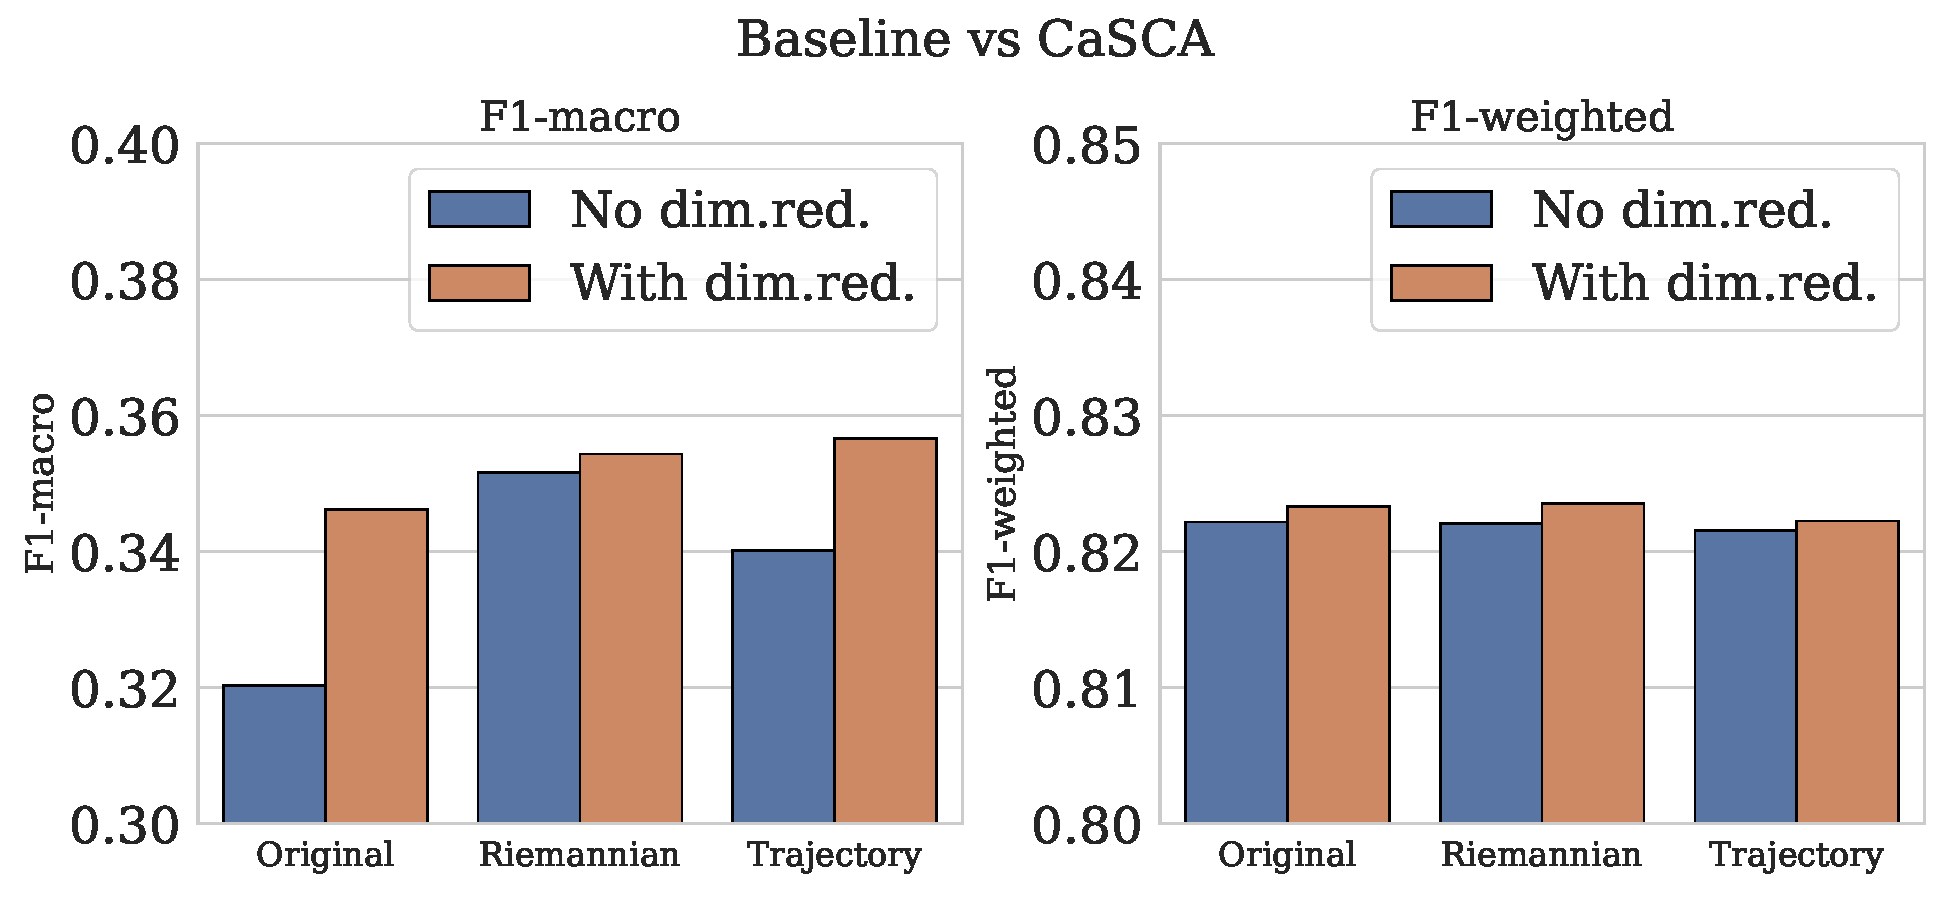
\includegraphics[width=.48\textwidth]{baseline-vs-casca.pdf}\label{fig:baseline-vs-casca}}
		\subfloat[]{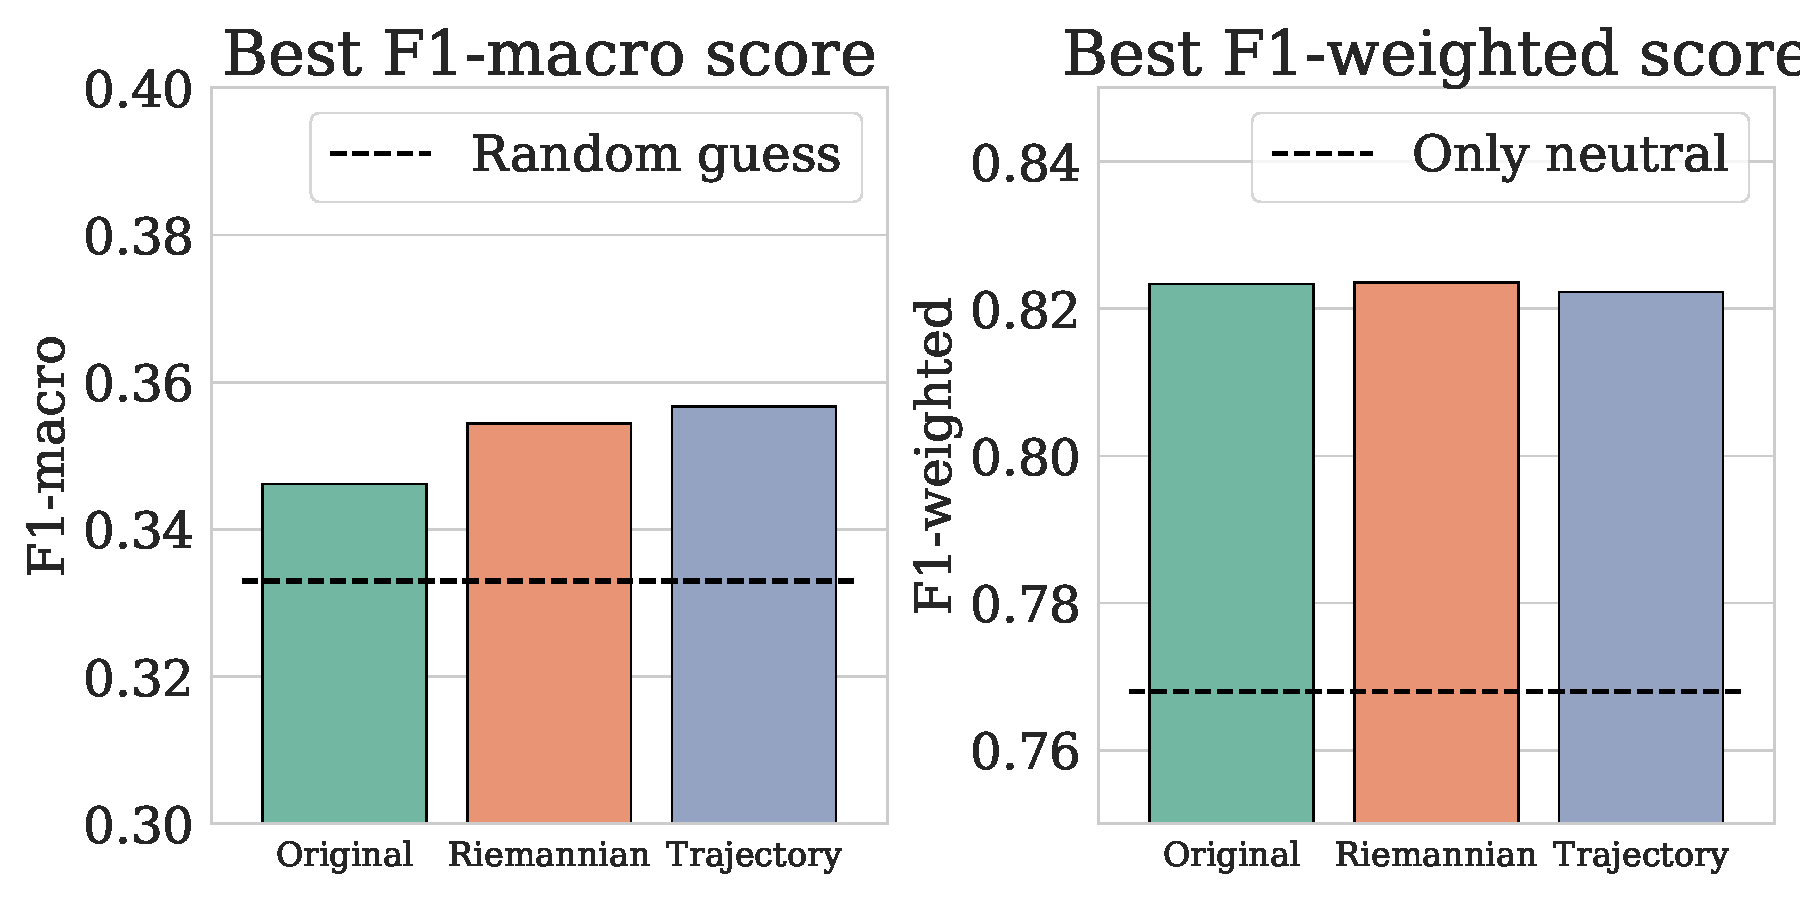
\includegraphics[width=.48\textwidth]{casca-spaces-baseline.pdf}\label{fig:casca-spaces-baseline}}
		\\
		\subfloat[]{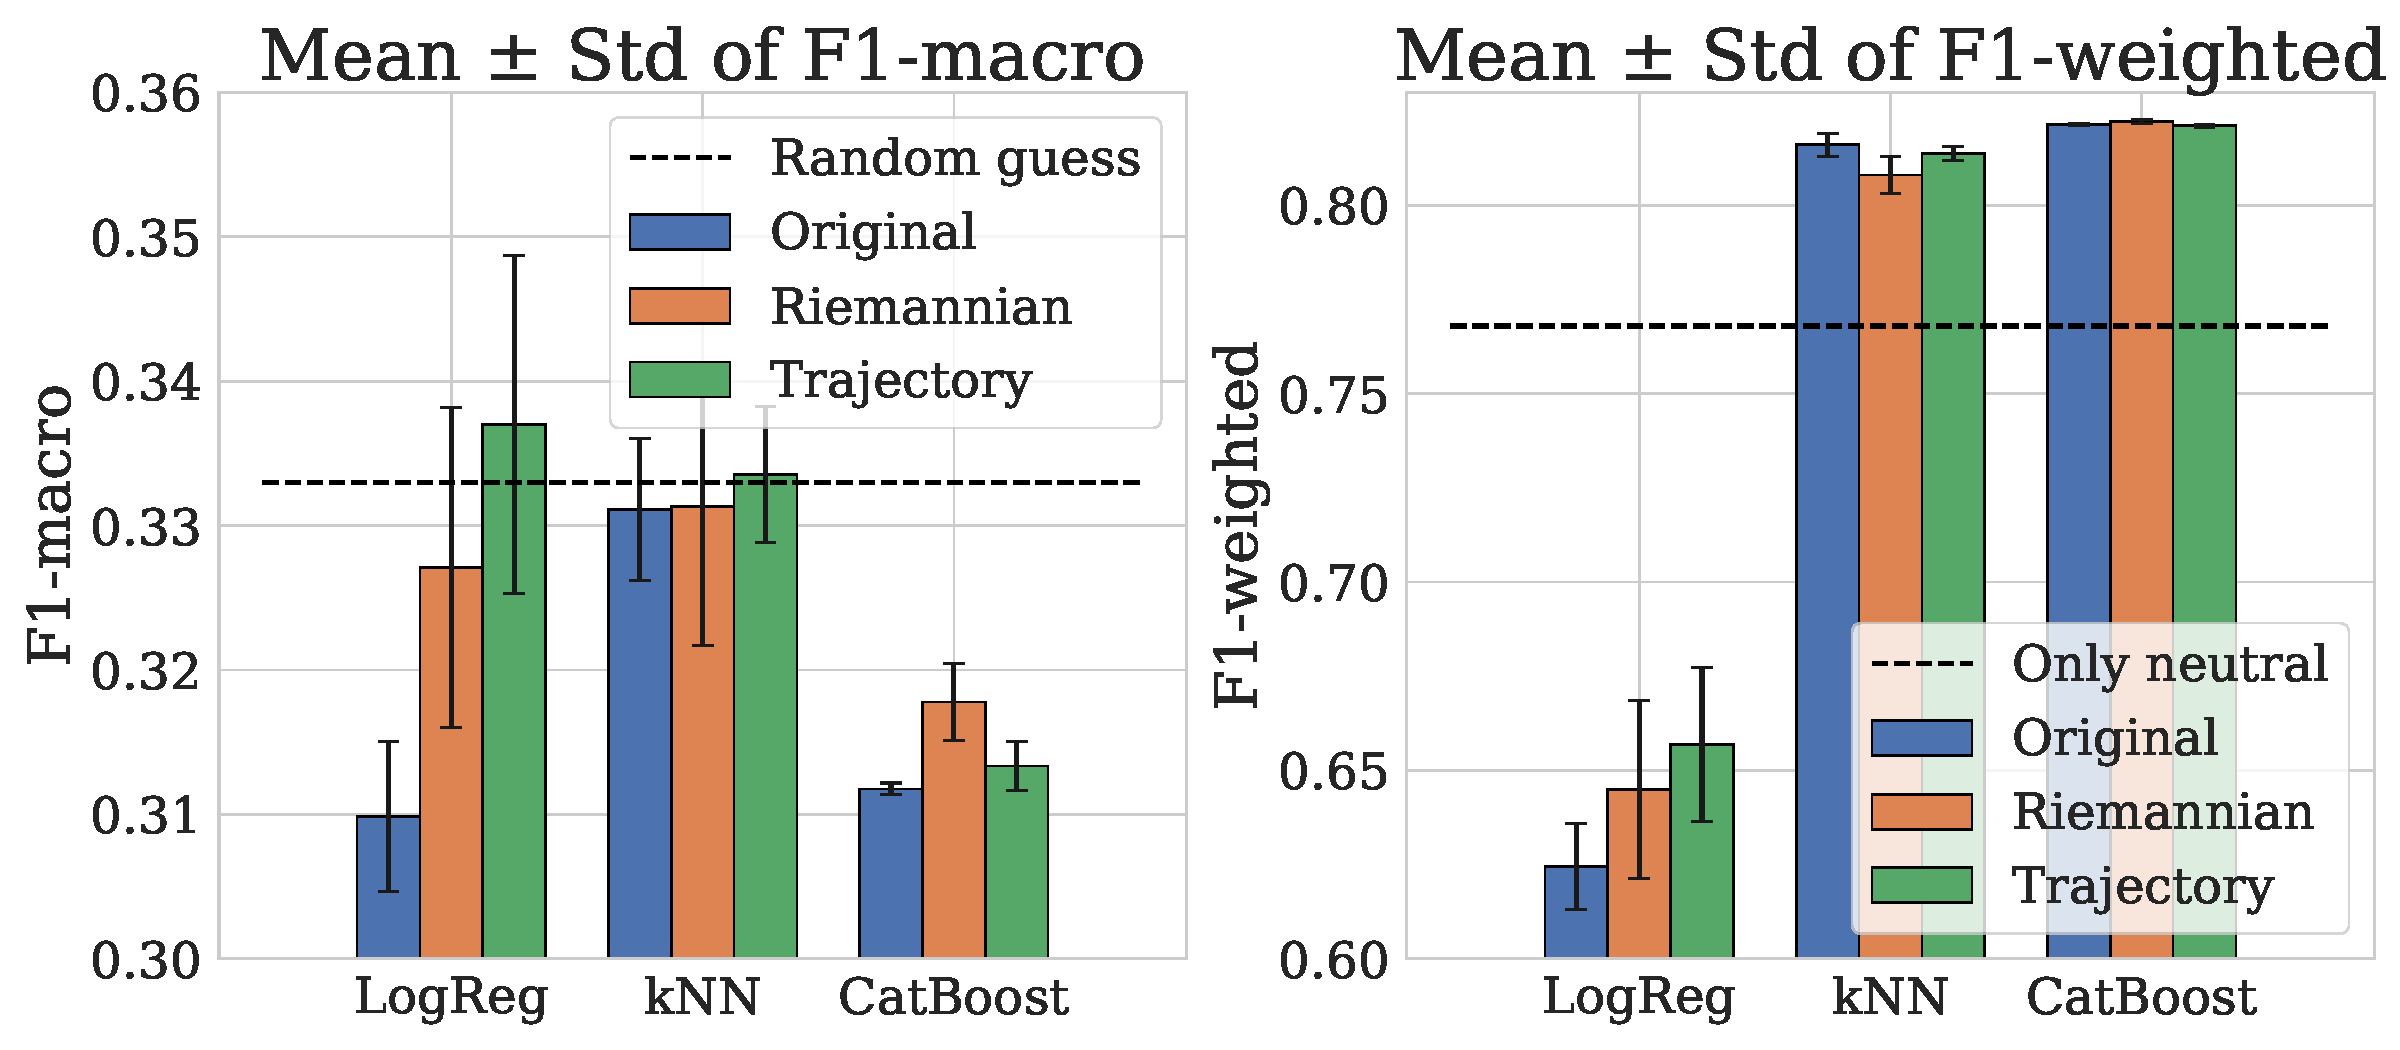
\includegraphics[width=.48\textwidth]{casca-spaces-by-models.pdf}\label{fig:casca-spaces-by-models}}
		\subfloat[]{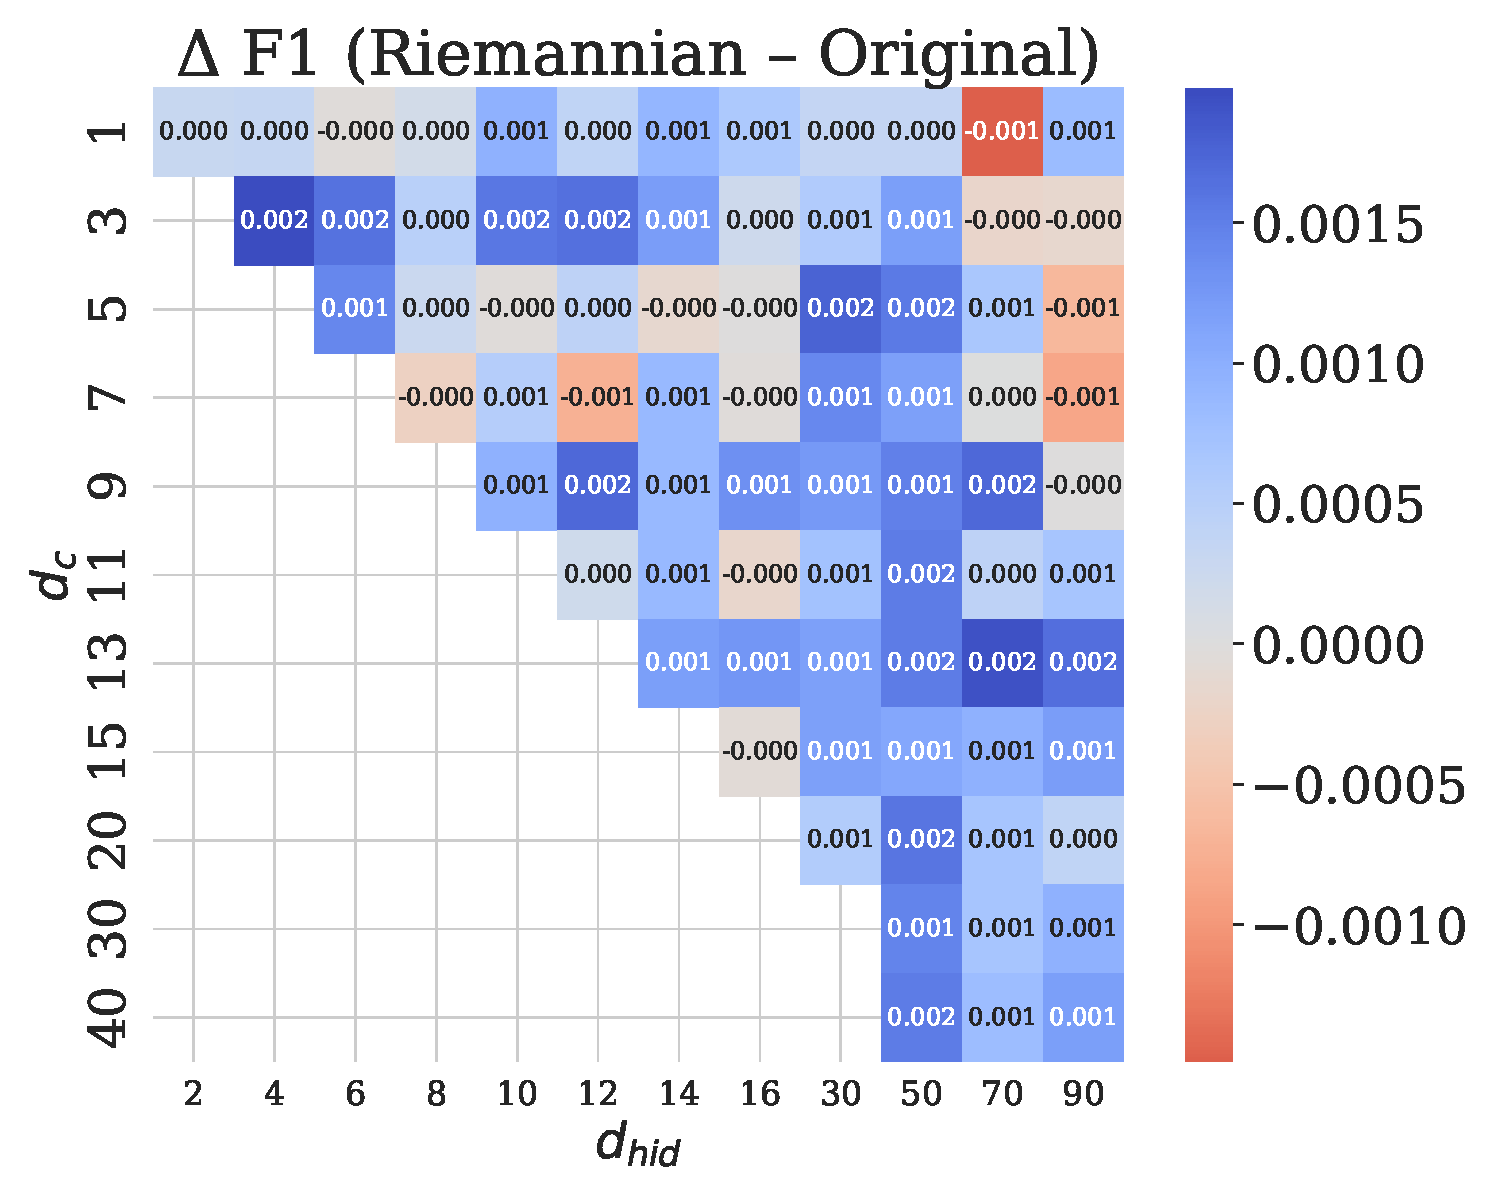
\includegraphics[width=.48\textwidth]{heatmap-delta-max_F1w-Riemannian-Original.pdf}\label{fig:heatmap-delta-max_F1w-Riemannian-Original}}
		\caption{EEG–IMU classification results.  
			(a) Baseline features vs.\ CaSCA embeddings.  
			(b) CaSCA vs.\ naive label priors.  
			(c) Mean $\pm$ sd macro-F$_1$ by classifier and observation space.  
			(d) F$_1$ gain of Riemannian over raw space.}
			\label{fig:eeg_imu_results}
	\end{figure}
	
	\paragraph{Baseline versus CaSCA.}
	Figure~\ref{fig:baseline-vs-casca} compares the best
	macro-F$_1$ of models trained only with EEG signals or only with IMU signals or with both type of signlas (blue bars) against the
	best score achieved with CaSCA embeddings (orange bars). Here we can see, that the prediction quality improves after applying CaSCA model 
	
	\paragraph{Which space is best?}
	Figure~\ref{fig:casca-spaces-baseline} shows that CaSCA vastly
	outperforms heuristic predictors (class priors or most-frequent
	class).  
	More importantly, CaSCA profits from appropriate geometry: in
	Fig.~\ref{fig:casca-spaces-by-models} the Riemannian SPD space
	consistently beats the raw domain and, for CatBoost, improves the mean
	macro-F$_1$ by $0.08$ with half the variance
	(see also the heat-map in
	Fig.~\ref{fig:heatmap-delta-max_F1w-Riemannian-Original}).
	
	\paragraph{CaSCA versus PurePCA / PureCCA.}
	Figure~\ref{fig:other_models} summarises how reconstruction fidelity, multicollinearity, and predictive accuracy respond to the choice of the causal dimension $d_c$ and the total hidden dimension $d_{\mathrm{hid}}=d_c+d_r$.  
	As expected, the explained–variance ratio grows almost monotonically with $d_{\mathrm{hid}}$ because every additional axis lets the decoder capture more signal energy; however, if one keeps $d_{\mathrm{hid}}$ fixed and allocates an excessive share to the causal block, reconstruction quality drops, reflecting the fact that purely causal directions cannot reproduce variance that is idiosyncratic to each sensor.  
	The variance–inflation factor shows the opposite trend: multicollinearity increases with larger $d_{\mathrm{hid}}$ since more latent axes are linearly related, and it grows especially fast when $d_c$ is large, confirming that the linear deflation\,+\,PCA back–end of CaSCA inflates cross-correlation when too many directions are forced into the causal span.  
	Predictive performance (macro-\(F_1\)) is highest for \emph{moderate} values of both $d_c$ and $d_{\mathrm{hid}}$; small latent spaces miss part of the interaction structure, whereas very large ones suffer from the amplified VIF, so downstream classifiers lose statistical power.  Altogether these curves support the empirical guideline used in the following sections: choose $d_c\!\in\!\{1,2\}$ and keep $d_{\mathrm{hid}}$ well below the raw channel count.
	
	\begin{figure}[bhtp]
		\centering
		\subfloat{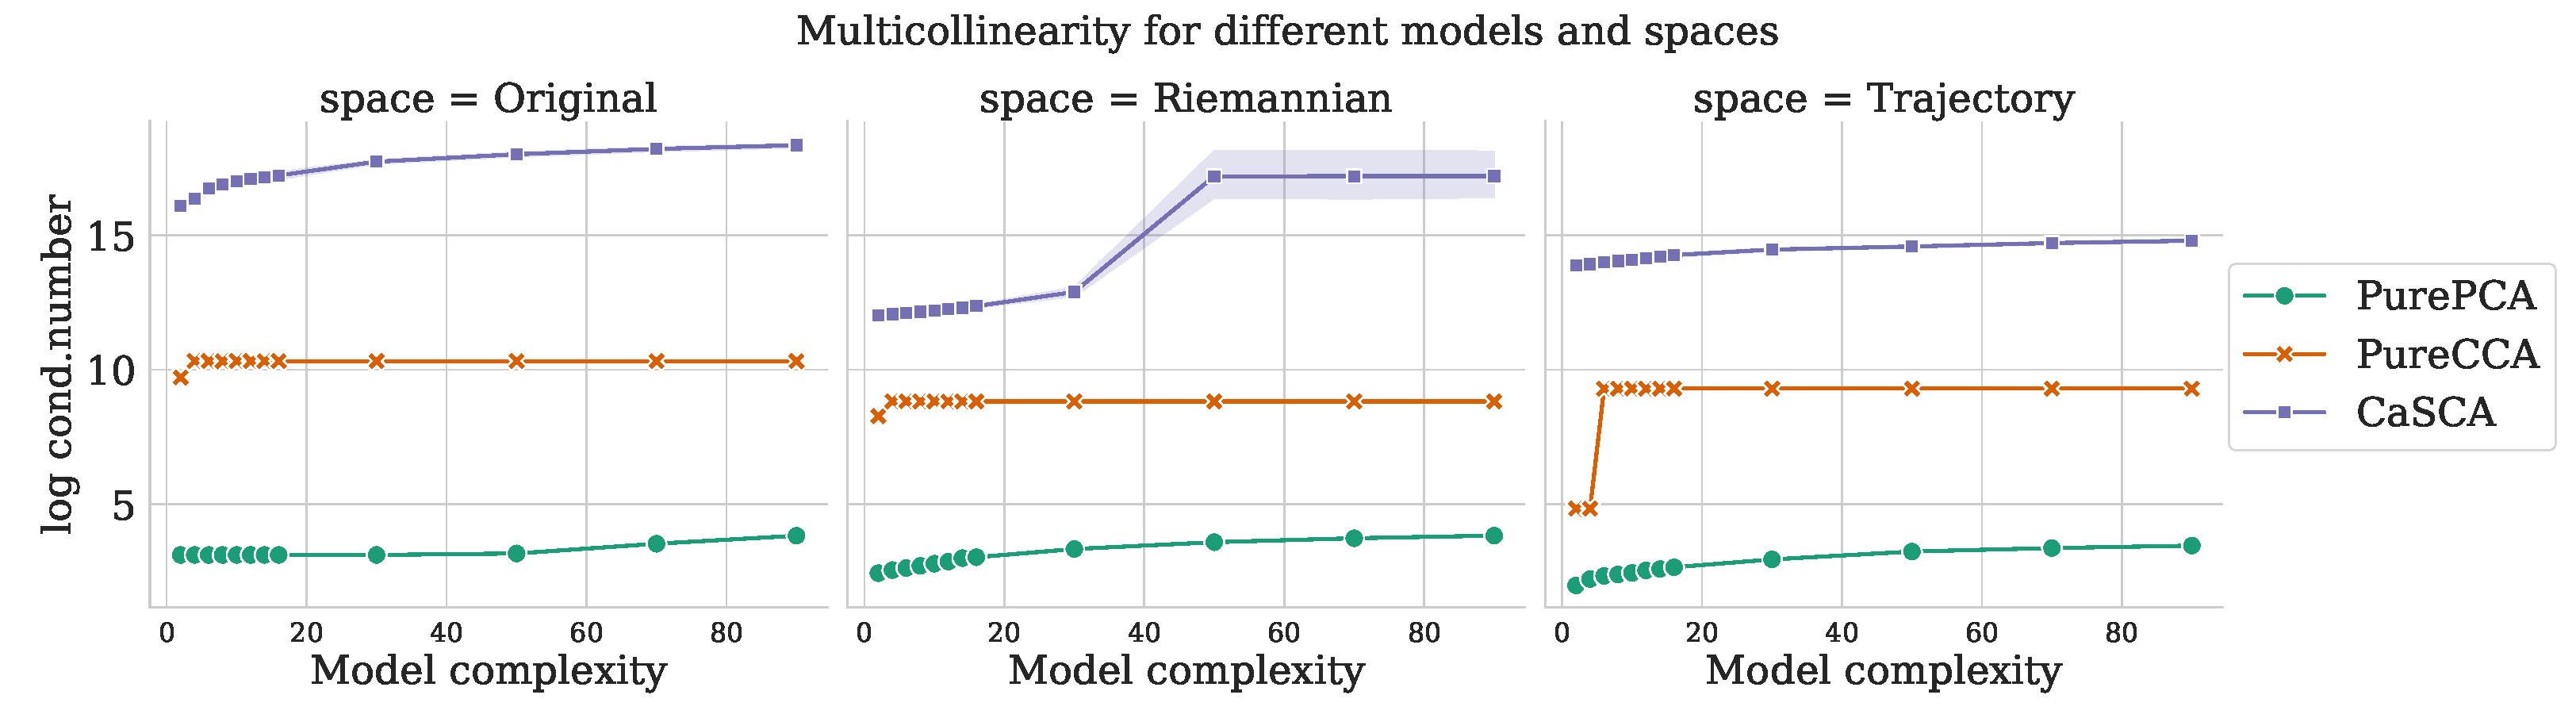
\includegraphics[width=0.9\linewidth]{other-models-multicollinearity.pdf}}\par
		\subfloat{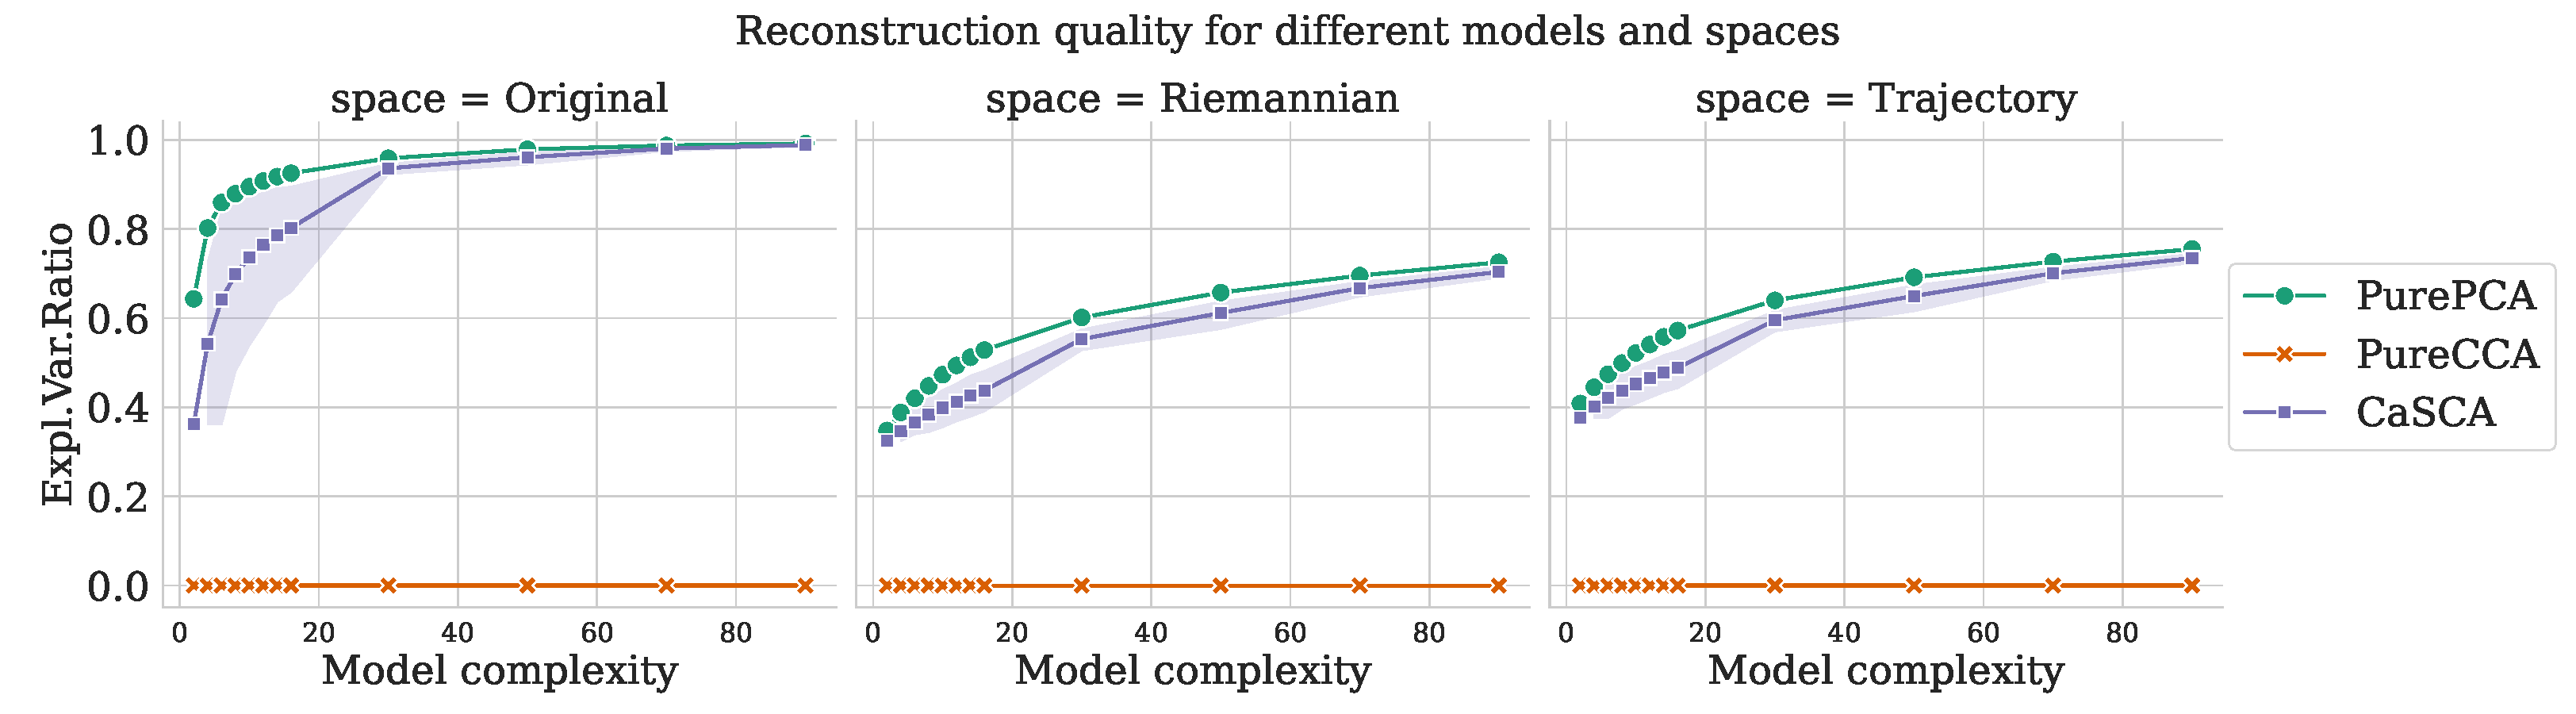
\includegraphics[width=0.9\linewidth]{other-models-reconstruction.pdf}}\par
		\subfloat{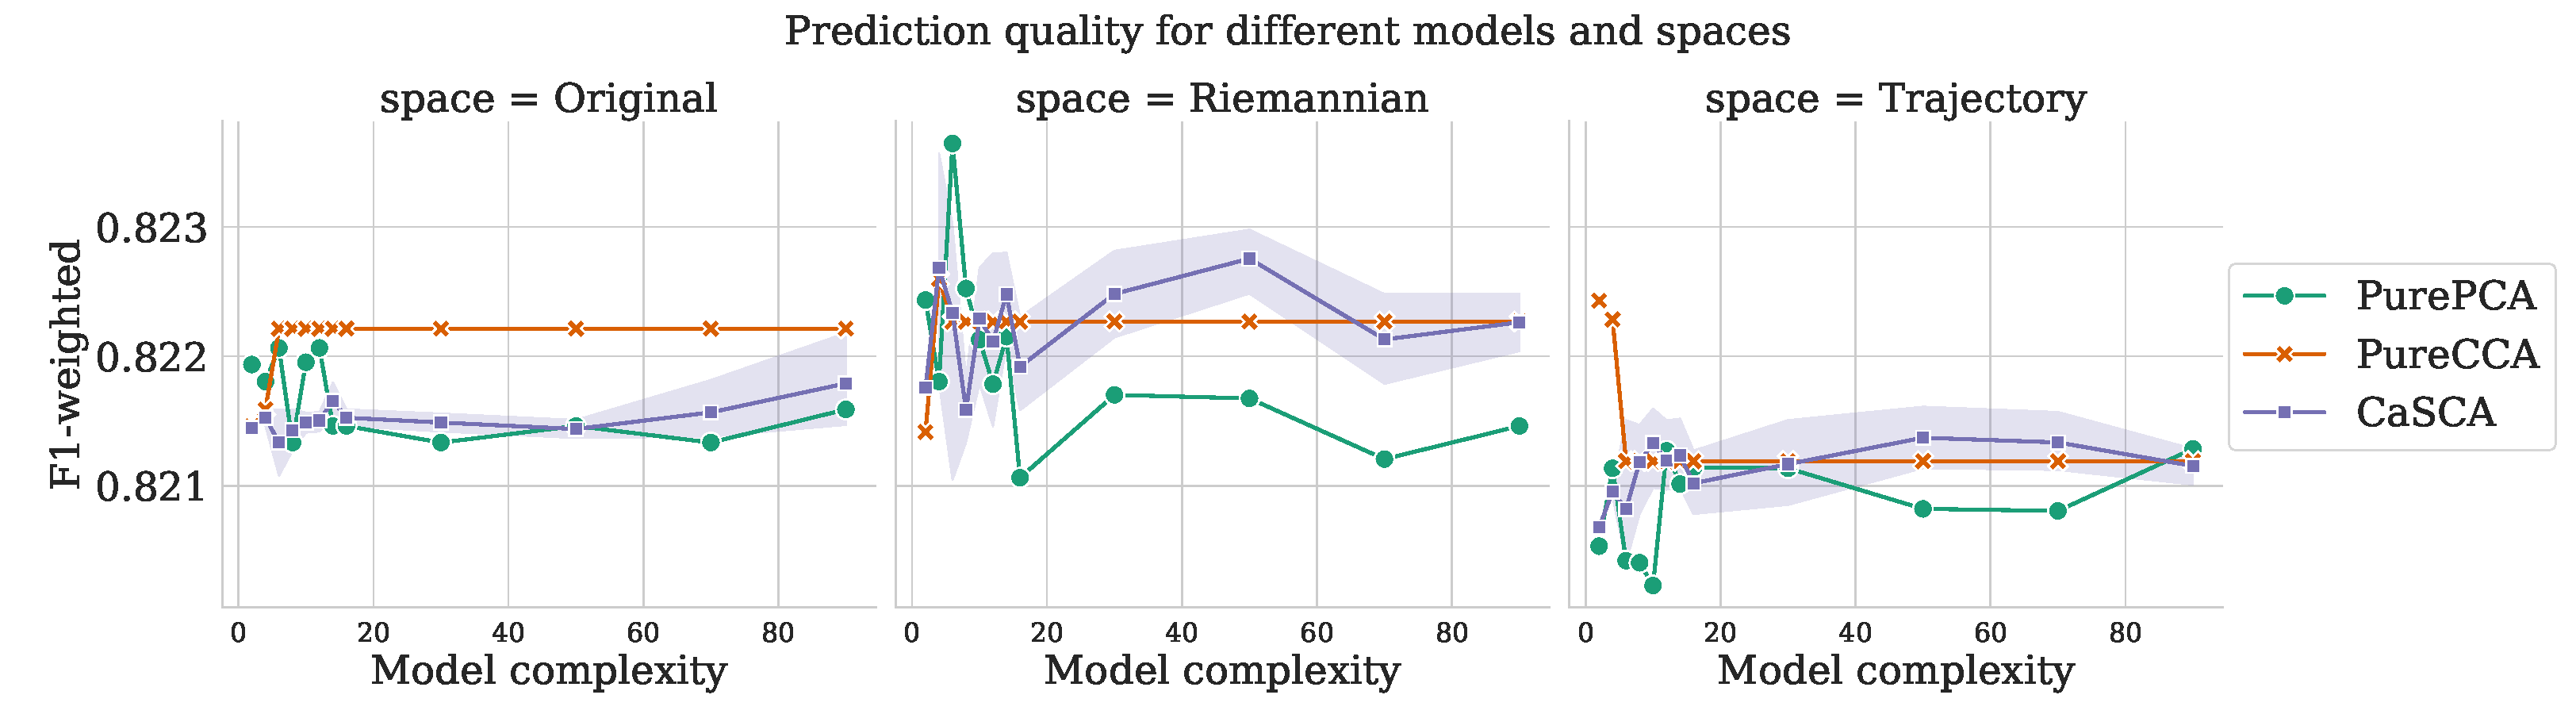
\includegraphics[width=0.9\linewidth]{other-models-prediction-f1-weighted.pdf}}
		\caption{Impact of latent dimensionality on (top) multicollinearity quality, (middle) reconstruction, and (bottom) weighted $F_1$ score.}
		\label{fig:other_models}
	\end{figure}

	\paragraph{Effect of causal and reconstruction dimensions.}
	\begin{figure}[bhtp]
		\centering
		\subfloat{\includegraphics[width=0.6\linewidth]{vif-–-trajectory-space}}\par
		\subfloat{\includegraphics[width=0.6\linewidth]{expl-var-ratio-–-trajectory-space.pdf}}\par
		\subfloat{\includegraphics[width=0.6\linewidth]{f1-macro-–-trajectory-space.pdf}}
		\caption{Relationship of $d_c$ and $d_{hid}$ in terms of (a) VIF score, (b) explained variance ratio and (c) macro F1-score}
		\label{fig:dc_and_dhid_relationship}
	\end{figure}

	Figure~\ref{fig:dc_and_dhid_relationship}
	jointly reveals how the choice of latent dimensions governs model behaviour.  
	First, the VIF heat-map (left panel) shows that multicollinearity increases almost linearly with $d_{\text{hid}}$.  
	Large latent spaces therefore risk unstable downstream regressions; the safest region lies at moderate sizes ($d_{\text{hid}}\!\approx\!6$–$8$), where VIF remains acceptable.  
	
	Second, the explained–variance curve (center panel) rises monotonically with the total hidden dimension $d_{\text{hid}}=d_c+d_r$, confirming that a broader latent space captures progressively more signal.  
	However, for any fixed $d_{\text{hid}}$ the curve bends downwards as the causal share $d_c$ grows: allocating too many dimensions to the causal block deprives the reconstructive block of capacity, reducing reconstruction fidelity.
	
	Finally, the macro-F1 surface (right panel) demonstrates a sweet-spot: predictive accuracy peaks for intermediate settings ($d_c=2$–$3$ and $d_{\text{hid}}=6$–$8$).  
	Too few dimensions ($d_{\text{hid}}\le 4$) fail to encode the cross-modal interaction, while too many ($d_{\text{hid}}\ge 10$) inflate multicollinearity and hurt generalisation.  
	Taken together, the graphics recommend \emph{moderate} latent sizes with a small causal share, balancing information retention, numerical stability, and predictive power across all embedding spaces examined.
	
	\paragraph{Take-aways.}
	\begin{itemize}
		\item Causal embeddings obtained with CaSCA improve classification even with small latent dimension;
		\item Working in delay or SPD-covariance space produces cleaner causal
		coordinates than the raw domain;
		\item CaSCA combines the reconstruction strength of PCA with the
		cross-view sensitivity of CCA, outperforming both when evaluated on
		real-world EEG–IMU data;
		\item Multicollinearity, measured by the maximum VIF, rises almost linearly with hidden space dimension;
		\item The highest F1-scores are achieved at intermediate latent sizes: models with too few dimensions miss cross-modal interactions, whereas overly large latents inflate VIF and degrade generalisation;
	\end{itemize}
	
%	\subsection{Metrics and Plots for 2-IMU}
%	
%	Figure 1 ("RMSE and $R^2$ vs $d_c, d_r$") shows that incorporating causal components ($d_c > 0$) consistently reduces prediction error.  
%	Figure 2 compares the performance of models trained in the original and trajectory spaces: all three metric groups (reconstruction, multicollinearity, predictive power) improve after switching to delays.  
%	Finally, Figure 3 illustrates the effect of lag optimization: models optimizing $\tau^\star$ show a substantial $R^2$ gain compared to $\tau = 0$.
	
	\section{Future Directions} \label{sec:future}
	
	The next stage of my research concentrates on two complementary ideas.  
	The first one aims at \emph{improving the existing pipeline} by incorporating explicit time‑varying dependencies.  
	Sequential locally weighted global linear maps (S‑maps) produce, at every observation time $t$, a Jacobian matrix $\mathbf J(t)=\bigl[\partial x_j(t+1)\!/\!\partial x_i(t)\bigr]_{i,j=1}^{d}$.  
	Each coefficient $J_{ij}(t)$ quantifies the instantaneous sensitivity of variable $X_j$ one step ahead to small perturbations of $X_i$ at the current state.  
	Treating the stochastic process $\{\mathbf J(t)\}_{t=1}^{T}$ as a first‑class data object allows us to embed local linear structure directly into causal discovery.   
	The result is a sequence of dynamic graphs whose adjacency matrices evolve as a function of the system’s position on the reconstructed manifold.  
	Such graphs reveal regime shifts, gradual drifts, and transient couplings that static mutual‑information scores inevitably obscure.  
	
	The second idea offers a new conceptual perspective by placing causal inference on an information‑geometric footing.  
	Let $\mathcal M_X$ and $\mathcal M_Y$ denote the statistical manifolds of probability measures on the measurable spaces of $X$ and $Y$, each endowed with the Fisher–Rao metric.  
	A causal mechanism “$X\!\rightarrow\!Y$’’ is formalised as a Markov kernel $\kappa(y\!\mid\!x)$ that induces the smooth map
	$$
	T_\kappa:\mathcal M_X\longrightarrow\mathcal M_Y,\qquad T_\kappa(P_X)=P_X\ast\kappa.
	$$
	Causal inference is reframed as estimating $T_\kappa$ or geometric properties from sample data drawn on $(X,Y)$.  
	Identifiability questions translate into the study of isometric between the two manifolds, while efficiency bounds emerge from comparison of Fisher–information tensors under $T_\kappa$.  
	This viewpoint unifies potential‑outcome, graphical, and dynamical formulations within a single coordinate‑free framework.  
	
	\section{Conclusion} \label{sec:conclusion}
	
	This work re-examined causal analysis through the lens of dimensionality reduction and proposed \textbf{CaSCA}: a two-block linear pipeline that first pinpoints lag-specific directions carrying predictive information from one multivariate signal to another, then compresses the residual variance into an orthogonal reconstructive basis.  
	By combining a grid search of shifted canonical-correlation pairs with exact Euclidean deflation, CaSCA guarantees that its causal and reconstructive loadings are mutually orthogonal once the data are whitened, yielding a clean block decomposition of the sample covariance and eliminating multicollinearity in downstream regressions.  
	We formalised these properties in a compact lemma–theorem package, showed how the latent scores reconstitute the original observations without overlap, and introduced three evaluation criteria—variance-inflation, reconstruction error, and predictive gain—that collectively diagnose whether a learned representation is both interpretable and useful.  
	Experiments on synthetic benchmarks, dual-sensor inertial recordings, and EEG–IMU data confirmed the method’s practical value: a small causal block consistently improved one-step forecasting and tennis-hit classification over baselines that operated either in the raw space or with unsupervised PCA/CCA.  
	The study also sketched extensions to trajectory embeddings, Riemannian manifolds, and a deep variant with a Convergent Cross-Mapping loss, suggesting a seamless upgrade path from linear algebra to modern representation learning.  
	Taken together, these contributions position CaSCA as a concise, theoretically grounded, and empirically effective foundation for future research in causal representation learning and state-space causal discovery.
	
	
	\addcontentsline{toc}{section}{\protect\numberline{}References}
	\bibliographystyle{unsrtnat}
	\bibliography{references.bib}
	
\end{document}
